\documentclass[12pt]{article}

\usepackage{hcmus-report-template}

% Disable indentation on new paragraphs
\setlength{\parindent}{0pt}
\setlength{\parskip}{4pt}

% Line spacing 1.5
\renewcommand{\baselinestretch}{1.5}

% Graphic path
\graphicspath{{images/}}

% To use Times font family, uncomment this row
% \usepackage{mathptmx}

% Define course name, report name and report title.
\newcommand{\coursename}{Introduction to Artificial Intelligence (CSC14003)}
\newcommand{\reportname}{Bloxorz Solver}
\newcommand{\reporttitle}{Project 1 Report}

% TODO: fill in the team members and the instructor.
\newcommand{\studentname}{%
  \fillin{Full name 1} -- \fillin{Student ID 1}\\
  \fillin{Full name 2} -- \fillin{Student ID 2}\\
  \fillin{Full name 3} -- \fillin{Student ID 3}\\
  \fillin{Full name 4} -- \fillin{Student ID 4}}
\newcommand{\teachername}{\fillin{Instructor name}}
\newcommand{\classname}{\fillin{Class}}

% Header
\lhead{\reporttitle}
\rhead{
University of Science - VNU-HCM\\
\coursename
}

% Footer
\newcommand{\leftfooter}{\LaTeX\ template by \href{https://github.com/trhgquan}{Quan, Tran Hoang}}
\lfoot{\footnotesize\leftfooter}

% ============ DOCUMENT ============
\begin{document}

\pagenumbering{roman}
% Cover page
\begin{titlepage}
\thispagestyle{empty}
\begin{center}
{\large\bfseries VIETNAM NATIONAL UNIVERSITY HO CHI MINH CITY\\
UNIVERSITY OF SCIENCE\\
FACULTY OF INFORMATION TECHNOLOGY\\}
\vspace{1.2cm}

% Put the HCMUS logo at images/hcmus-logo.png; it is skipped while the file is missing.
\IfFileExists{images/hcmus-logo.png}{%
  \includegraphics[width=0.32\linewidth]{hcmus-logo.png}\\[1.2cm]
}{\vspace{3cm}}

{\Huge\bfseries \reporttitle\\[0.4cm]}
{\Large Topic: \reportname\\[0.2cm]}
{\large Course: \coursename\\}
\vspace{1.5cm}

\begin{tabular}{rl}
\textbf{Students:} & \begin{tabular}[t]{@{}l@{}}\studentname\end{tabular}\\[0.4cm]
\textbf{Class:} & \classname\\[0.2cm]
\textbf{Instructor:} & \teachername\\
\end{tabular}

\vfill
{\large Ho Chi Minh City, \today}
\end{center}
\end{titlepage}


\tableofcontents
\pagebreak
\listoftables
\pagebreak
\listoffigures
\pagebreak

\pagenumbering{arabic}
\setcounter{page}{1}

\section{Project Planning and Task Distribution}

\subsection{Team members}

\begin{table}[H]
\centering
\caption{Team members}
\label{tab:members}
\begin{tabular}{clll}
\toprule
\textbf{No.} & \textbf{Full name} & \textbf{Student ID} & \textbf{Email} \\
\midrule
1 & \fillin{Full name 1} & \fillin{ID} & \fillin{Email} \\
2 & \fillin{Full name 2} & \fillin{ID} & \fillin{Email} \\
3 & \fillin{Full name 3} & \fillin{ID} & \fillin{Email} \\
4 & \fillin{Full name 4} & \fillin{ID} & \fillin{Email} \\
\bottomrule
\end{tabular}
\end{table}

\subsection{Timeline}

\begin{table}[H]
\centering
\caption{Project timeline}
\label{tab:timeline}
\begin{tabularx}{\linewidth}{lX}
\toprule
\textbf{Period} & \textbf{Milestones} \\
\midrule
\fillin{Week 1} & \fillin{Game state, transition table, level format, core mechanics, GUI skeleton} \\
\fillin{Week 2} & \fillin{Advanced tiles (fragile, bridges, soft/heavy/split switches); BFS and DFS solvers} \\
\fillin{Week 3} & \fillin{UCS and A* solvers, test levels, experiments, report and demo video} \\
\bottomrule
\end{tabularx}
\end{table}

\subsection{Task distribution}

Each member's completion percentage is used to compute the individual score
(individual score $=$ group score $\times$ completion percentage).

\begin{table}[H]
\centering
\caption{Task distribution and completion}
\label{tab:tasks}
\begin{tabularx}{\linewidth}{Xll}
\toprule
\textbf{Task} & \textbf{Assigned to} & \textbf{Completion} \\
\midrule
Game core mechanics (board, block orientations, rolling, win/lose) & \fillin{Member} & \fillin{\%} \\
Advanced tiles (fragile, bridges, soft/heavy/split switches) & \fillin{Member} & \fillin{\%} \\
GUI (Panda3D scene, controls, solver buttons, playback) & \fillin{Member} & \fillin{\%} \\
Level format and test levels (JSON, level generator) & \fillin{Member} & \fillin{\%} \\
BFS solver & \fillin{Member} & \fillin{\%} \\
DFS solver & \fillin{Member} & \fillin{\%} \\
UCS solver and cost function & \fillin{Member} & \fillin{\%} \\
A* solver and heuristic & \fillin{Member} & \fillin{\%} \\
Experiments, tables and charts & \fillin{Member} & \fillin{\%} \\
Report & \fillin{Member} & \fillin{\%} \\
Demo video & \fillin{Member} & \fillin{\%} \\
\bottomrule
\end{tabularx}
\end{table}

\begin{table}[H]
\centering
\caption{Completion percentage of each member}
\label{tab:completion}
\begin{tabular}{lc}
\toprule
\textbf{Member} & \textbf{Completion} \\
\midrule
\fillin{Full name 1} & \fillin{\%} \\
\fillin{Full name 2} & \fillin{\%} \\
\fillin{Full name 3} & \fillin{\%} \\
\fillin{Full name 4} & \fillin{\%} \\
\bottomrule
\end{tabular}
\end{table}

\subsection{Requirement checklist}

\begin{table}[H]
\centering
\caption{Self-evaluation against the project requirements}
\label{tab:checklist}
\begin{tabularx}{\linewidth}{Xcl}
\toprule
\textbf{Requirement} & \textbf{Points} & \textbf{Status} \\
\midrule
Reimplement the game: core mechanics & 10 & Completed \\
Reimplement the game: advanced tiles & 10 & Completed \\
BFS solver & 10 & Completed \\
DFS solver & 10 & Completed (DFS, not IDS) \\
UCS solver & 10 & Completed \\
A* solver & 10 & Completed \\
Report & 30 & \fillin{Status} \\
Demo video & 10 & \fillin{Status} \\
\bottomrule
\end{tabularx}
\end{table}

\section{Project Overview}

\subsection{The game}

Bloxorz is a block-rolling puzzle. The player rolls a $1\times1\times2$ block over a grid of
tiles and must drop it, standing upright, into a goal hole. The block can stand on one cell
or lie horizontally or vertically across two cells, and a roll fails if any part of the block
ends up over a void cell or outside the board. Our implementation supports every tile type of
the assignment: floor, void, goal, fragile tiles, bridges, and soft, heavy and split switches
with both \emph{toggle} and \emph{permanent} bridge behaviour, including splitting the block
into two cubes and merging them again.

\subsection{Implementation}

The program is written in Python 3.10+ with a Panda3D desktop GUI. The code is organised in
four layers whose dependencies point strictly downwards, so the solvers never depend on the GUI
(Table~\ref{tab:modules}).

\begin{table}[H]
\centering
\caption{Source code organisation}
\label{tab:modules}
\begin{tabularx}{\linewidth}{lX}
\toprule
\textbf{Module} & \textbf{Responsibility} \\
\midrule
\texttt{models/} & Immutable search states (\texttt{BlockState}, \texttt{GameState}), the \texttt{Level} data and the validated JSON level loader. \\
\texttt{engine/transitions.py} & The game rules: orientation table, legality, switches, bridges, split and merge, \texttt{successors()} and \texttt{is\_goal()}. \\
\texttt{solvers/} & \texttt{bfs.py}, \texttt{dfs.py}, \texttt{ucs.py}, \texttt{astar.py}; \texttt{common.py} holds \texttt{SearchResult} and the shared cost function. \\
\texttt{gui/} & Panda3D scene, input, animations, solver buttons and solution playback. \\
\texttt{levels/} & \texttt{campaign.json} and 35 levels (\texttt{test1.json} to \texttt{test34.json}, \texttt{test\_all.json}). \\
\bottomrule
\end{tabularx}
\end{table}

\textbf{Level format.} Each stage is a JSON file, so the same stage is reused by the GUI and
by all four solvers. The \texttt{map} field is a list of strings using the symbols
\texttt{\#} (void), \texttt{.} (floor), \texttt{S}/\texttt{G} (start/goal), \texttt{F} (fragile),
\texttt{B} (bridge), \texttt{o} (soft switch), \texttt{X} (heavy switch) and \texttt{P}
(split switch). Optional lists define bridge groups (cells and initial state), switches
(position, type, \texttt{toggle} or \texttt{permanent}, target bridges) and split switches
(position and the two destination cells). Every level is validated when the program starts.

\textbf{GUI.} The window shows the 3D board, the block and every tile type. The control bar has
\emph{New Game} (level selector) and \emph{Restart} buttons, and one button per solver
(\emph{BFS}, \emph{DFS}, \emph{UCS}, \emph{A*}). A solver runs from the current state; a results
card then shows Search Time, Memory Usage, Expanded Nodes and Solution Length, and the solution is
replayed with Play, Pause, Step Back and Step Forward controls.

\textbf{Running the program.} From the \texttt{Source/} folder:
\begin{lstlisting}[language=bash, numbers=none]
python -m pip install -r requirements.txt
python main.py
\end{lstlisting}

\section{Algorithm Description}

\subsection{Formalising the search problem}

Bloxorz is fully observable and deterministic: the whole board is visible and each action
leads to exactly one successor. We therefore model it as a classical search problem. All four
solvers share the same problem definition and never re-implement the game rules; they only call
\texttt{successors(level, state)} and \texttt{is\_goal(level, state)} from
\texttt{engine/transitions.py}. A rule therefore lives in one place and affects every algorithm
in the same way, which keeps the comparison fair.

\subsubsection{State representation}

The static stage (tiles, goal, switch definitions) is stored in a \texttt{Level} object and is
\emph{not} part of the state. A state is an immutable \texttt{GameState}
(Table~\ref{tab:state}).

\begin{table}[H]
\centering
\caption{Components of a search state}
\label{tab:state}
\begin{tabularx}{\linewidth}{llX}
\toprule
\textbf{Field} & \textbf{Type} & \textbf{Meaning} \\
\midrule
\texttt{block.orientation} & \texttt{S}, \texttt{H}, \texttt{V} & Standing, lying horizontally, lying vertically \\
\texttt{block.row}, \texttt{block.col} & int & \texttt{S}: occupied cell; \texttt{H}: left cell; \texttt{V}: top cell \\
\texttt{bridge\_mask} & int (bitmask) & Bit $i$ is 1 when bridge group $i$ is open \\
\texttt{cubes} & \texttt{None} or two cells & Positions of the two cubes after a split \\
\texttt{active\_cube} & 0 or 1 & The cube that the next move controls \\
\bottomrule
\end{tabularx}
\end{table}

\begin{itemize}[leftmargin=*]
\item \textbf{Orientation} is part of the state because it decides which cells are occupied,
whether the block may rest on a fragile tile, whether it can win, and how each roll transforms it.
\item \textbf{Bridge configuration} is part of the state, as required: the same block placement
with different open/closed bridges allows different moves. A bitmask keeps the state small and
fast to hash; with $B$ bridge groups there are at most $2^B$ configurations.
\item \textbf{Split mode} needs \texttt{cubes} and \texttt{active\_cube}; the active cube decides
which cube the next action moves.
\item \texttt{GameState} is a frozen dataclass, hence hashable, so whole states are used as
dictionary keys and set members to detect repeated states.
\end{itemize}

For a stage with $N$ floor cells, an unsplit block has at most about $3N$ placements, multiplied
by $2^B$ bridge configurations; split mode adds at most $2N(N-1)$ cube configurations. Our test
stages have 37 to 90 floor cells and at most two bridge groups, so only hundreds to a few thousand
states are reachable; the \emph{Test All} stage (432 floor cells, six bridge groups, a split
switch) is much larger.

\subsubsection{Initial state and goal test}

The initial state is the state passed to the solver: the GUI passes the current state, which may
be mid-level, split, or have bridges toggled; the experiments use the stage's start state (block
standing on \texttt{S}, bridges as defined in the JSON file). The goal test holds only when the
block is whole, \emph{standing}, and on the goal cell. A block lying across the goal and a single
cube do not win.

\subsubsection{Actions and transition model}

The actions are \texttt{UP}, \texttt{DOWN}, \texttt{LEFT}, \texttt{RIGHT} and, only while the
block is split, \texttt{SWAP}. \texttt{transition(level, state, action)} returns the next state
or \texttt{None} for an illegal move, in five steps.

\textbf{(1) Orientation table.} Table~\ref{tab:roll} lists the twelve deterministic
(orientation, direction) cases. A standing block tips over in the rolling direction, a block
lying along the rolling direction stands up, and a block lying across it rolls sideways.

\begin{table}[H]
\centering
\caption{Orientation transition table, block at $(r,c)$}
\label{tab:roll}
\begin{tabular}{lllll}
\toprule
\textbf{From} & \textbf{UP} & \textbf{DOWN} & \textbf{LEFT} & \textbf{RIGHT} \\
\midrule
\texttt{S} & \texttt{V} $(r-2,c)$ & \texttt{V} $(r+1,c)$ & \texttt{H} $(r,c-2)$ & \texttt{H} $(r,c+1)$ \\
\texttt{H} & \texttt{H} $(r-1,c)$ & \texttt{H} $(r+1,c)$ & \texttt{S} $(r,c-1)$ & \texttt{S} $(r,c+2)$ \\
\texttt{V} & \texttt{S} $(r-1,c)$ & \texttt{S} $(r+2,c)$ & \texttt{V} $(r,c-1)$ & \texttt{V} $(r,c+1)$ \\
\bottomrule
\end{tabular}
\end{table}

\textbf{(2) Legality.} Every occupied cell must be supported (not void, not off the board, not a
closed bridge), and a standing block must not be on a fragile tile.

\textbf{(3) Switches} fire only on a fresh press (pressed after the move but not before it).
A soft switch fires when any part of the block, or a cube, covers it; a heavy switch only when
the block stands on it. A \emph{toggle} effect flips the bridge bits (XOR); a \emph{permanent}
effect sets them to a fixed state.

\textbf{(4) Split.} A block that arrives standing on a split switch is teleported into two cubes
at predefined cells (optionally changing bridges). Each move then moves the active cube by one
cell; cubes can press soft switches only.

\textbf{(5) Merge.} When the two cubes become adjacent they merge into an \texttt{H} or
\texttt{V} block, if that placement is legal.

Illegal moves never appear in \texttt{successors()}, so no solver generates a falling state.

\subsubsection{Cost function}

BFS and DFS ignore costs. UCS and A* share the risk-aware cost \texttt{move\_cost} defined in
\texttt{solvers/common.py} (Table~\ref{tab:cost}).

\begin{table}[H]
\centering
\caption{Step cost used by UCS and A*}
\label{tab:cost}
\begin{tabular}{lc}
\toprule
\textbf{Transition} & \textbf{Cost} \\
\midrule
\texttt{SWAP} & 0 \\
Each roll of the block or step of a cube & 1 \\
Additional penalty if any occupied cell ends on a fragile tile & $+4$ \\
\bottomrule
\end{tabular}
\end{table}

\begin{itemize}[leftmargin=*]
\item \textbf{Why not uniform.} With a cost of 1 per move, UCS reduces to BFS. We make risky
moves expensive instead.
\item \textbf{Fragile penalty.} A fragile tile breaks if the block ends up standing on it, so a
path that keeps landing on fragile tiles is one wrong orientation away from failure. A penalty of
4 means the solver accepts a detour of up to three extra rolls to avoid one fragile landing. It is
large enough to change the path when a detour exists and small enough that unavoidable fragile
tiles are still crossed.
\item \textbf{SWAP is free} because it moves nothing; it only changes which cube is controlled.
This also matches the GUI's Moves counter, which does not count \texttt{SWAP}.
\item \textbf{Consequences.} All costs are non-negative, which UCS and A* need for optimality,
and every non-\texttt{SWAP} move costs at least 1, which the A* heuristic relies on
(Section~\ref{sec:heuristic}). UCS and A* minimise risk-weighted cost, not the number of moves;
the number of moves is still reported separately.
\end{itemize}

\subsubsection{Avoiding repeated states}

All four algorithms are graph searches and always compare the \emph{whole} \texttt{GameState},
never just coordinates (Table~\ref{tab:visited}). The state space is finite and each state is
expanded at most once, so no algorithm can loop. Two consecutive zero-cost \texttt{SWAP}s return
to a state that is already closed, so they cannot loop either. A dictionary
\texttt{parents[state] = (previous\_state, action)} rebuilds the solution by walking back from the
goal and reversing the actions.

\begin{table}[H]
\centering
\caption{Repeated-state handling}
\label{tab:visited}
\begin{tabular}{lll}
\toprule
\textbf{Algorithm} & \textbf{Structure} & \textbf{State marked when} \\
\midrule
BFS & \texttt{parents} dictionary & generated \\
DFS & \texttt{parents} dictionary & popped from the stack \\
UCS, A* & \texttt{best} cost dictionary $+$ \texttt{closed} set & popped from the priority queue \\
\bottomrule
\end{tabular}
\end{table}

\subsubsection{Measurements}

Every solver returns a \texttt{SearchResult} with the four required measurements:
\textbf{search time} (\texttt{time.perf\_counter()} around the search loop),
\textbf{peak memory} (the peak of Python allocations during the search, from
\texttt{tracemalloc}), \textbf{expanded nodes} (the number of states whose successors were
generated) and \textbf{solution length} (the number of moves, \texttt{SWAP} excluded).

% -------------------------------------------------------------------------
\subsection{Breadth-First Search (BFS)}

BFS expands states level by level: first every state one action away from the start, then every
state two actions away, and so on. The frontier is a FIFO queue (\texttt{collections.deque}).

\begin{algorithm}[H]
\caption{BFS (\texttt{solvers/bfs.py})}
\label{alg:bfs}
\begin{algorithmic}[1]
\If{\Call{IsGoal}{$start$}} \Return empty path \EndIf
\State $parents \gets \{start: \textsc{None}\}$; $frontier \gets$ queue $[start]$
\While{$frontier$ is not empty}
  \State $s \gets frontier.\textsc{PopLeft}()$; $expanded \gets expanded + 1$
  \For{each $(a, s')$ in \Call{Successors}{$s$}}
    \If{$s' \in parents$} \textbf{continue} \EndIf
    \State $parents[s'] \gets (s, a)$
    \If{\Call{IsGoal}{$s'$}} \Return \Call{Rebuild}{$parents, s'$} \Comment{goal test on generation}\EndIf
    \State $frontier.\textsc{Append}(s')$
  \EndFor
\EndWhile
\State \Return no solution
\end{algorithmic}
\end{algorithm}

\begin{itemize}[leftmargin=*]
\item \texttt{parents} doubles as the visited set, so every state enters the queue once.
\item The goal test is applied when a state is \emph{generated}. With BFS the first generated goal
is always at minimum depth, so stopping early keeps optimality and saves a whole layer of
expansions.
\item \textbf{Complete}: the state space is finite. \textbf{Optimal in the number of actions},
\texttt{SWAP} included. It does not guarantee the fewest displayed moves (10 moves $+$ 3
\texttt{SWAP} $=$ 13 actions loses to 11 moves $+$ 0 \texttt{SWAP}) and it ignores fragile tiles.
\item Time and memory $O(b^d)$, where $b \le 4$ ($5$ when split) is the branching factor and $d$
the solution depth; in practice bounded by the number of reachable states.
\end{itemize}

% -------------------------------------------------------------------------
\subsection{Depth-First Search (DFS)}

We implement \textbf{graph-search DFS} (not IDS). DFS always follows the newest branch until it
gets stuck, then backtracks. The frontier is a LIFO stack.

\begin{algorithm}[H]
\caption{DFS (\texttt{solvers/dfs.py})}
\label{alg:dfs}
\begin{algorithmic}[1]
\State $parents \gets \{\}$; $stack \gets [(start, \textsc{None})]$
\While{$stack$ is not empty}
  \State $(s, link) \gets stack.\textsc{Pop}()$
  \If{$s \in parents$} \textbf{continue} \EndIf
  \State $parents[s] \gets link$ \Comment{marked when popped}
  \If{\Call{IsGoal}{$s$}} \Return \Call{Rebuild}{$parents, s$} \EndIf
  \State $expanded \gets expanded + 1$
  \For{each $(a, s')$ in \textsc{Reversed}(\Call{Successors}{$s$})}
    \If{$s' \notin parents$} $stack.\textsc{Push}((s', (s, a)))$ \EndIf
  \EndFor
\EndWhile
\State \Return no solution
\end{algorithmic}
\end{algorithm}

\begin{itemize}[leftmargin=*]
\item An explicit stack replaces recursion, so long paths (1363 moves on Test All) cannot hit
Python's recursion limit.
\item A state is marked when \emph{popped}, not when pushed, so the recorded parent link is the
route DFS actually followed to it.
\item Successors are pushed in reverse so that the engine's first action (\texttt{UP}, then
\texttt{DOWN}, \texttt{LEFT}, \texttt{RIGHT}, \texttt{SWAP}) is explored first.
\item \textbf{Complete} on a finite space thanks to the visited set, but \textbf{not optimal}: it
returns the first solution it meets. The frontier stays small ($O(b\,m)$ for maximum depth $m$),
although the visited set can grow to the size of the state space.
\end{itemize}

% -------------------------------------------------------------------------
\subsection{Uniform-Cost Search (UCS)}

UCS expands the state with the smallest path cost $g(n)$ first. The frontier is a binary heap
(\texttt{heapq}) keyed on $g$.

\begin{algorithm}[H]
\caption{UCS (\texttt{solvers/ucs.py})}
\label{alg:ucs}
\begin{algorithmic}[1]
\State $best \gets \{start: 0\}$; $parents \gets \{start: \textsc{None}\}$; $closed \gets \emptyset$
\State $heap \gets [(0, 0, tie, start)]$ \Comment{(cost, number of actions, insertion order, state)}
\While{$heap$ is not empty}
  \State $(g, depth, \_, s) \gets heap.\textsc{PopMin}()$
  \If{$s \in closed$} \textbf{continue} \Comment{stale entry}\EndIf
  \If{\Call{IsGoal}{$s$}} \Return \Call{Rebuild}{$parents, s$} \Comment{goal test on pop}\EndIf
  \State $closed \gets closed \cup \{s\}$; $expanded \gets expanded + 1$
  \For{each $(a, s')$ in \Call{Successors}{$s$}}
    \If{$s' \in closed$} \textbf{continue} \EndIf
    \State $g' \gets g + \Call{MoveCost}{s, s', a}$
    \If{$s' \notin best$ \textbf{or} $g' < best[s']$}
      \State $best[s'] \gets g'$; $parents[s'] \gets (s, a)$
      \State $heap.\textsc{Push}((g', depth + 1, tie, s'))$
    \EndIf
  \EndFor
\EndWhile
\State \Return no solution
\end{algorithmic}
\end{algorithm}

\begin{itemize}[leftmargin=*]
\item \textbf{Goal test on pop.} With non-uniform costs, the goal may first be generated through
an expensive route; only when it is popped is its $g$ guaranteed minimal.
\item \textbf{Lazy deletion.} \texttt{heapq} has no decrease-key, so a cheaper route pushes a new
entry and the old one is skipped when popped (it is already in \texttt{closed}).
\item \textbf{Tie-breaking.} Among equal costs, fewer actions are preferred; the insertion counter
prevents Python from comparing two \texttt{GameState} objects.
\item \textbf{Complete and optimal} with respect to \texttt{move\_cost}, because all step costs are
non-negative. Time $O(N \log N)$ and memory $O(N)$, where $N$ is the number of states cheaper than
the optimal cost $C^*$. UCS grows in cost contours, so when the solution must cross a fragile tile
it also expands states deeper than the solution depth.
\end{itemize}

% -------------------------------------------------------------------------
\subsection{A* Search}

A* uses the same skeleton and the same cost $g$ as UCS, but orders the heap by
\begin{equation}
f(n) = g(n) + h(n),
\end{equation}
where $h(n)$ estimates the remaining cost. The heap key is $(f, h, \text{insertion order})$, so
among equal $f$ the state closer to the goal is preferred. Because $h$ is consistent
(Section~\ref{sec:admissible}), each state can be closed on its first expansion without reopening.

\subsubsection{Heuristic design}
\label{sec:heuristic}

\textbf{Idea: a lower bound on moving the block's centre.} Ignore terrain, fragile tiles, bridges
and orientation legality, and ask only how many rolls are needed to move the block's centre to the
goal's centre. Coordinates are doubled (half-cell units) so that centres are integers
(Table~\ref{tab:centre}); the goal is a standing block on $G=(g_r, g_c)$, with centre
$(2g_r, 2g_c)$.

\begin{table}[H]
\centering
\caption{Block centre in doubled coordinates}
\label{tab:centre}
\begin{tabular}{ll}
\toprule
\textbf{Shape} & \textbf{Centre} \\
\midrule
\texttt{S} at $(r,c)$ & $(2r, 2c)$ \\
\texttt{H} at $(r,c)$ & $(2r, 2c+1)$ \\
\texttt{V} at $(r,c)$ & $(2r+1, 2c)$ \\
Two cubes at $(r_0,c_0), (r_1,c_1)$ & $(r_0+r_1, c_0+c_1)$ \\
\bottomrule
\end{tabular}
\end{table}

In these units, a roll changes only one coordinate; standing $\leftrightarrow$ lying shifts the
centre by 3 (1.5 cells) and lying $\to$ lying by 2; a cube step shifts the cubes' midpoint by 1;
\texttt{SWAP} shifts nothing. Every move of cost $\ge 1$ therefore moves the centre by at most 3 in
Manhattan distance, which gives
\begin{equation}
\mathrm{direct}(p, q) = \left\lceil \frac{|p_r - q_r| + |p_c - q_c|}{3} \right\rceil .
\end{equation}
This is the assignment's ``Manhattan distance divided by 2'' idea, tightened to 1.5 cells per roll.
It is also orientation-aware without an extra term: a lying block's centre sits half a cell off the
grid, so a lying block next to the goal still gets $h \ge 1$.

\textbf{Split switches.} A split switch teleports the block, so $\mathrm{direct}(p, \text{goal})$
alone could overestimate. For each split switch $q$ with entry $E_q$ (its \texttt{P} tile) and exit
$X_q$ (the midpoint of its destination cubes), the code computes $T[q]$, the best bound from $X_q$
to the goal, possibly through other switches, by Bellman--Ford style relaxation over the few
switches. The heuristic is
\begin{equation}
h(p) = \min\Big( \mathrm{direct}(p, \text{goal}),\ \min_q \big[\mathrm{direct}(p, E_q) + T[q]\big] \Big),
\end{equation}
treating the teleport as free, which can only lower the bound.

\subsubsection{Admissibility and consistency}
\label{sec:admissible}

The heuristic must be admissible with respect to our cost function, \texttt{move\_cost}.

\textbf{Admissible.} A path to the goal either never fires a split switch or fires one. In the
first case each move shifts the centre by at most 3, so at least $\mathrm{direct}(p,\text{goal})$
moves are needed, each costing at least 1. In the second case at least
$\mathrm{direct}(p, E_q)$ moves come before the teleport and at least $T[q]$ after it, by the same
argument from the exit. \texttt{SWAP} costs 0 but does not move the centre, and the fragile penalty
only increases the true cost. Hence $h(n) \le h^*(n)$ for every state.

\textbf{Consistent} ($h(s) \le c(s,s') + h(s')$ for every edge):
\begin{itemize}[leftmargin=*]
\item \emph{Roll or cube step:} $\mathrm{direct}$ satisfies the triangle inequality because
$\lceil (a+b)/3 \rceil \le \lceil a/3 \rceil + \lceil b/3 \rceil$, and one move shifts the centre by
at most 3, so $h(s) \le 1 + h(s') \le c + h(s')$ for any $c \ge 1$, including penalised moves.
\item \emph{SWAP:} the centre is unchanged, so $h(s) = h(s')$ and $c = 0$.
\item \emph{Teleport:} $h(s) \le \mathrm{direct}(p, E_q) + T[q] \le 1 + h(s')$, since $T[q]$ is
exactly the heuristic value at the exit.
\end{itemize}
A consistent heuristic is also admissible, and lets A* close each state once while remaining
optimal. The experiments agree: A* and UCS return the same cost on all 34 test stages.

\subsubsection{Limitations}

The bound ignores terrain, so it is loose on winding maps where the real path must detour, and it
prices every move at 1, so it underestimates when fragile tiles cannot be avoided. A tighter
admissible alternative would be a relaxed point-on-grid BFS distance computed once per stage.

% -------------------------------------------------------------------------
\subsection{Summary}

\begin{table}[H]
\centering
\caption{Theoretical comparison of the four algorithms}
\label{tab:theory}
\begin{tabularx}{\linewidth}{lXXXX}
\toprule
 & \textbf{BFS} & \textbf{DFS} & \textbf{UCS} & \textbf{A*} \\
\midrule
Frontier & FIFO queue & LIFO stack & heap on $g$ & heap on $g+h$ \\
Goal test & on generation & on pop & on pop & on pop \\
Complete & yes & yes (finite space) & yes & yes \\
Optimal for & number of actions & -- & \texttt{move\_cost} & \texttt{move\_cost} \\
Uses cost / heuristic & no / no & no / no & yes / no & yes / yes \\
Time & $O(b^d)$ & $O(b^m)$ & $O(b^{1+\lfloor C^*/\epsilon \rfloor})$ & depends on $h$ \\
\bottomrule
\end{tabularx}
\end{table}

\section{Experiments}

\subsection{Setup}

Each solver was run once on each test stage, starting from the stage's initial state. The runs
are produced by \texttt{experiments/run\_experiments.py}, which writes
\texttt{experiments/summary\_4\_metrics.csv}; the charts are drawn from that file by
\texttt{experiments/plot\_results.py} (pandas, matplotlib and seaborn). The algorithms are
deterministic: re-running the experiment reproduces exactly the same expanded nodes, solution
lengths and paths. Search time and memory depend on the machine, and time is inflated several times
by \texttt{tracemalloc}, so they are meaningful only \emph{relative to each other}.

\begin{table}[H]
\centering
\caption{Measured quantities}
\label{tab:metrics}
\begin{tabularx}{\linewidth}{llX}
\toprule
\textbf{Metric} & \textbf{Unit} & \textbf{How it is measured} \\
\midrule
Search time & ms & \texttt{time.perf\_counter()} around the search loop \\
Memory usage & KB & Peak traced allocation during the search (\texttt{tracemalloc}) \\
Expanded nodes & states & States whose successors were generated \\
Solution length & moves & Rolls and cube steps, \texttt{SWAP} excluded \\
\bottomrule
\end{tabularx}
\end{table}

\subsection{Test set}

We use a fixed set of 34 stages, \texttt{test1.json} to \texttt{test34.json}, identical for all
algorithms. Stages 1--9 were designed by hand; stages 10--34 were generated by
\texttt{experiments/generate\_levels.py} with fixed seeds, and each generated stage was accepted
only if it loads, belongs to the requested group, is solvable by BFS and has a long enough
solution. The stages are grouped automatically from their content into four groups of increasing
difficulty (Table~\ref{tab:groups}). The \emph{Test All} stage, which combines every mechanic on a
much larger map, is reported separately as a stress test.

\begin{table}[H]
\centering
\caption{Test groups}
\label{tab:groups}
\begin{tabularx}{\linewidth}{lXcl}
\toprule
\textbf{Group} & \textbf{Mechanics} & \textbf{Stages} & \textbf{Stage numbers} \\
\midrule
G1 Basic & Floor, void and goal only & 6 & 1, 10--14 \\
G2 Fragile & Adds 1--4 fragile tiles & 6 & 2, 15--19 \\
G3 Bridges \& Switches & Bridges with soft/heavy switches (toggle and permanent), no fragile tiles & 15 & 3--5, 7, 8, 20--24, 30--34 \\
G4 Combined & Fragile tiles and switches; Test 9 also has a split switch & 7 & 6, 9, 25--29 \\
Stress test & All mechanics: 6 bridge groups, 5 switches, a split switch; 432 floor cells & 1 & Test All \\
\bottomrule
\end{tabularx}
\end{table}

The 34 stages range from $12\times25$ to $25\times15$ cells (one $15\times35$), with 37 to 90
floor cells each.

\subsection{Results}

\subsubsection{Summary tables}

Table~\ref{tab:overall} averages each metric over the 34 stages. ``Risk cost'' is the
\texttt{move\_cost} of the returned path (moves $+\,4\times$ fragile landings), the quantity UCS and
A* minimise; ``Moves / BFS'' is the solution length divided by the BFS solution length on the same
stage.

\begin{table}[H]
\centering
\caption{Mean over the 34 test stages}
\label{tab:overall}
\small\setlength{\tabcolsep}{4pt}
\begin{tabular}{lrrrrrr}
\toprule
\textbf{Algorithm} & \textbf{Time (ms)} & \textbf{Memory (KB)} & \textbf{Expanded} & \textbf{Moves} & \textbf{Risk cost} & \textbf{Moves / BFS} \\
\midrule
BFS & 47.68 & 33.45 & 179.5 & 22.79 & 25.62 & 1.00 \\
DFS & 35.92 & 25.90 & 125.2 & 74.18 & 79.71 & 3.34 \\
UCS & 55.93 & 52.05 & 194.4 & 22.97 & \textbf{24.97} & 1.01 \\
A*  & \textbf{30.16} & 31.54 & \textbf{97.4} & 22.97 & \textbf{24.97} & 1.01 \\
\bottomrule
\end{tabular}
\end{table}

Medians are less sensitive to the outlier Test 9: expanded nodes BFS 147, DFS 123, UCS 150.5,
A* 92.5; moves BFS 22.5, DFS 73.5, UCS 23, A* 23.

\begin{table}[H]
\centering
\caption{Mean per test group}
\label{tab:bygroup}
\begin{tabular}{llrrrr}
\toprule
\textbf{Group} & \textbf{Algorithm} & \textbf{Time (ms)} & \textbf{Memory (KB)} & \textbf{Expanded} & \textbf{Moves} \\
\midrule
\multirow{4}{*}{G1 Basic} & BFS & 30.36 & 22.09 & 121.7 & 22.17 \\
 & DFS & 23.36 & 21.50 & 103.2 & 56.17 \\
 & UCS & 28.71 & 33.65 & 125.8 & 22.17 \\
 & A* & 16.76 & 21.94 & 66.7 & 22.17 \\
\midrule
\multirow{4}{*}{G2 Fragile} & BFS & 26.95 & 19.05 & 104.0 & 20.83 \\
 & DFS & 22.39 & 17.37 & 82.7 & 55.67 \\
 & UCS & 31.49 & 32.82 & 118.0 & 21.33 \\
 & A* & 21.19 & 24.79 & 73.5 & 21.33 \\
\midrule
\multirow{4}{*}{\shortstack[l]{G3 Bridges\\\& Switches}} & BFS & 53.02 & 35.99 & 196.0 & 23.80 \\
 & DFS & 43.18 & 30.91 & 149.9 & 91.20 \\
 & UCS & 66.79 & 57.78 & 206.4 & 23.80 \\
 & A* & 34.54 & 34.01 & 106.1 & 23.80 \\
\midrule
\multirow{4}{*}{G4 Combined} & BFS & 68.83 & 50.09 & 258.3 & 22.86 \\
 & DFS & 42.72 & 26.26 & 127.7 & 69.00 \\
 & UCS & 76.91 & 72.05 & 293.1 & 23.29 \\
 & A* & 39.94 & 40.26 & 125.3 & 23.29 \\
\bottomrule
\end{tabular}
\end{table}

\begin{table}[H]
\centering
\caption{Stress test on Test All (measured separately; time and memory on a different machine)}
\label{tab:testall}
\begin{tabular}{lrrrrr}
\toprule
\textbf{Algorithm} & \textbf{Time (ms)} & \textbf{Memory (KB)} & \textbf{Expanded} & \textbf{Moves} & \textbf{SWAP} \\
\midrule
BFS & 369.7 & 1457.2 & 5838 & 84 & 2 \\
DFS & 138.0 & 834.5 & 2519 & 1363 & 47 \\
UCS & 415.2 & 2527.9 & 6398 & 84 & 2 \\
A*  & 188.4 & 941.6 & 2610 & 84 & 2 \\
\bottomrule
\end{tabular}
\end{table}

Per-stage results for all 34 stages are listed in Appendix~\ref{app:perlevel}.

\subsubsection{Charts}

\begin{figure}[H]
\centering
\begin{subfigure}{0.49\linewidth}
  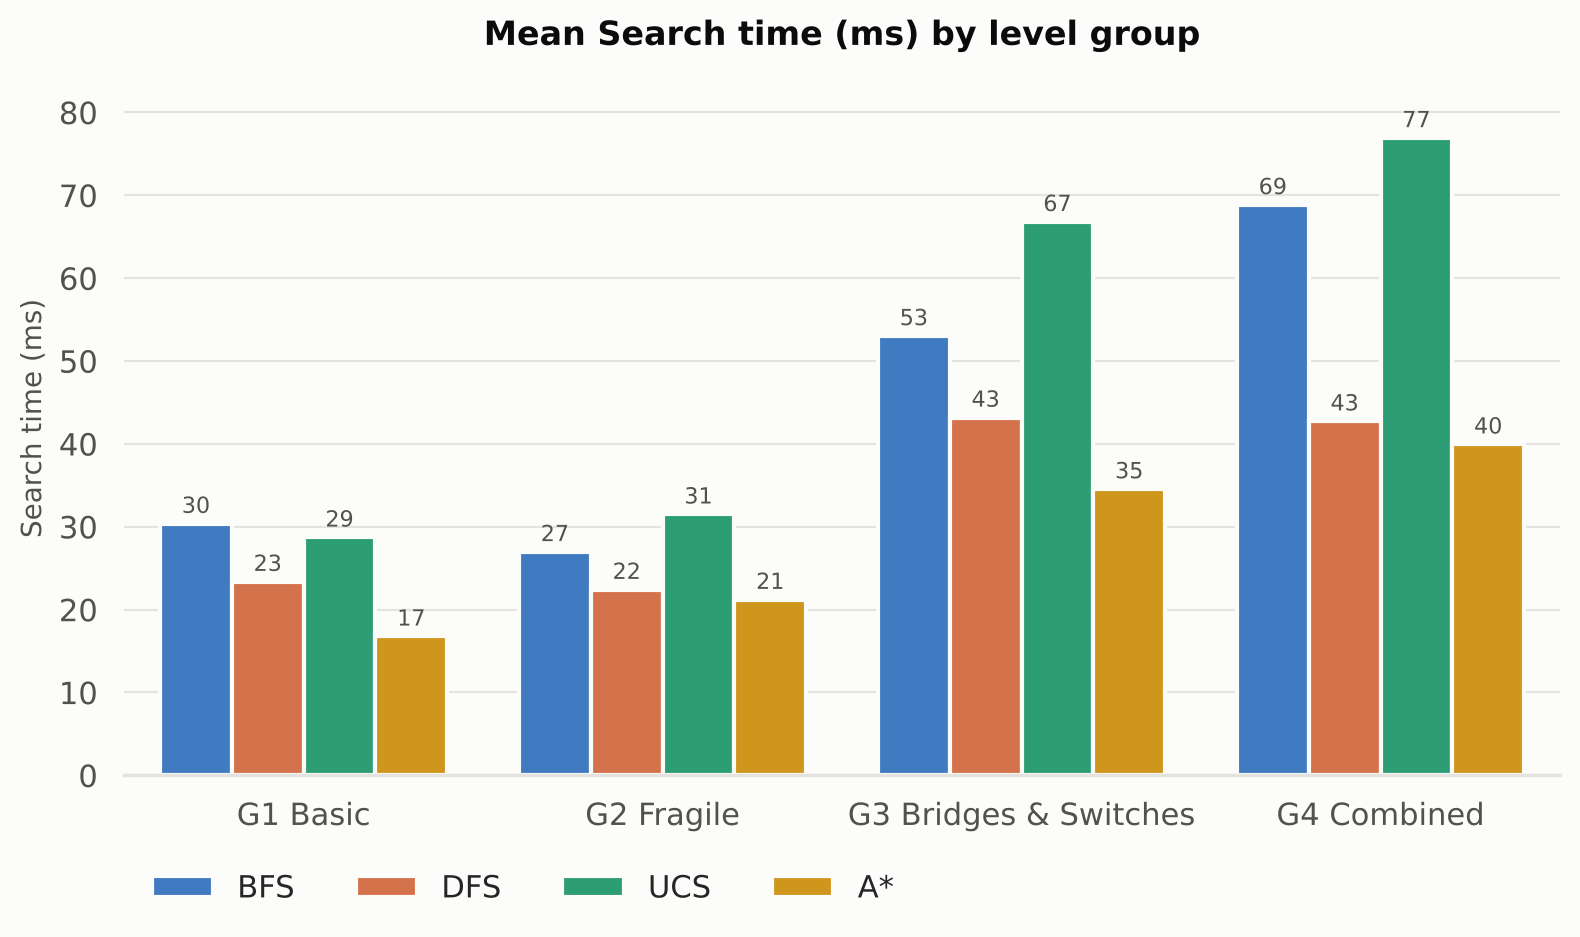
\includegraphics[width=\linewidth]{fig1a_time_by_group.png}
  \caption{Search time}
\end{subfigure}
\hfill
\begin{subfigure}{0.49\linewidth}
  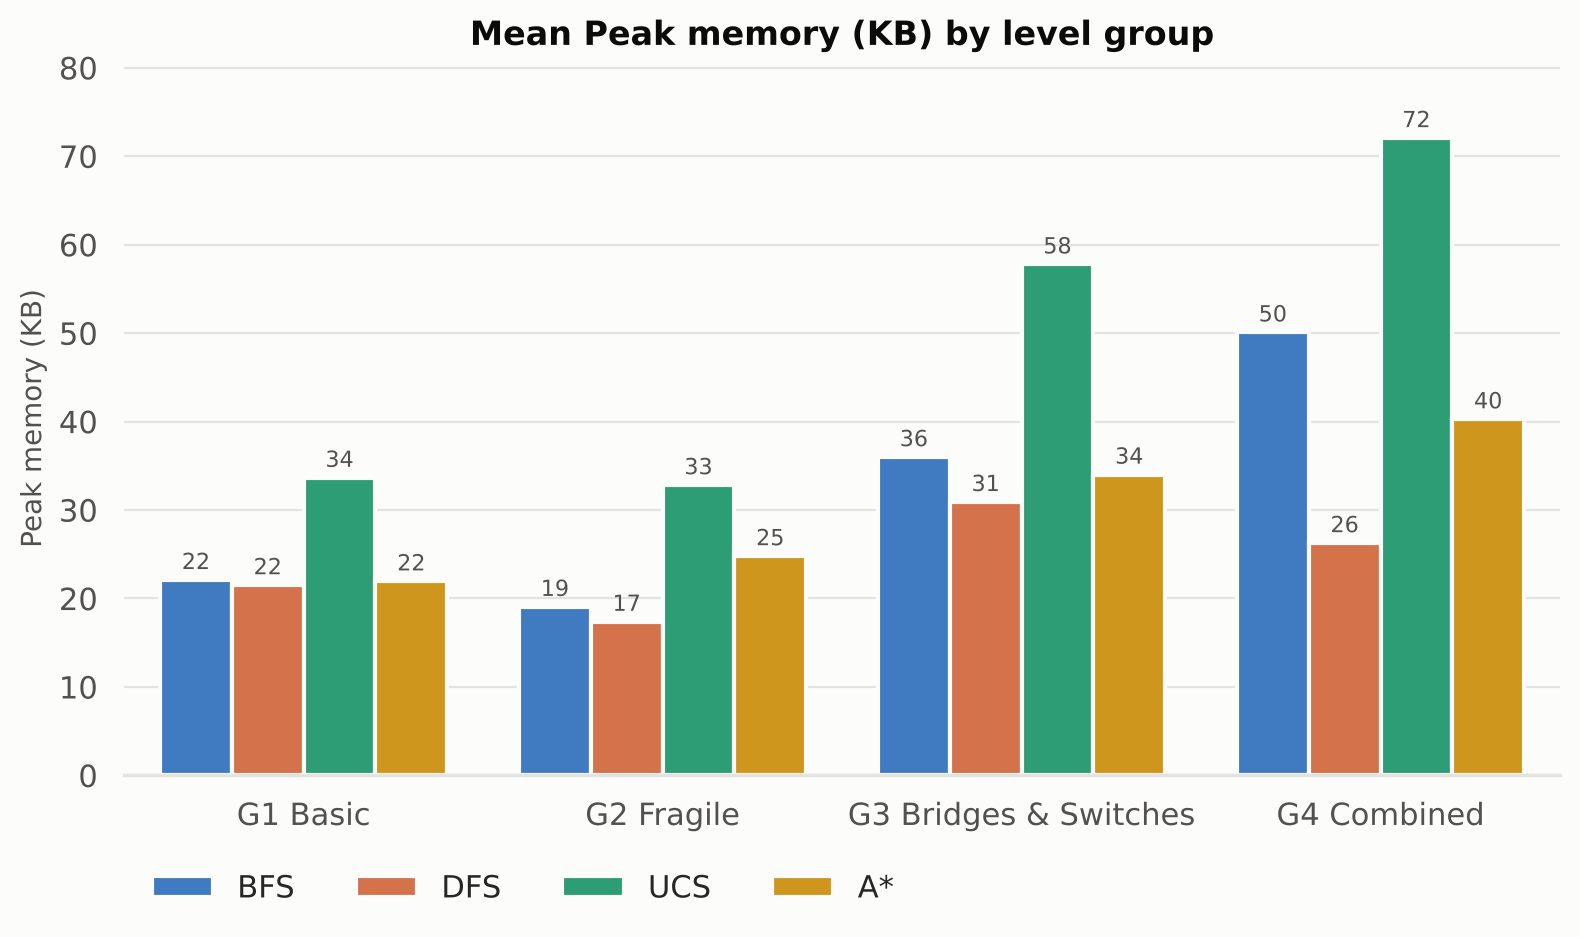
\includegraphics[width=\linewidth]{fig1b_memory_by_group.png}
  \caption{Peak memory}
\end{subfigure}
\\[0.3cm]
\begin{subfigure}{0.49\linewidth}
  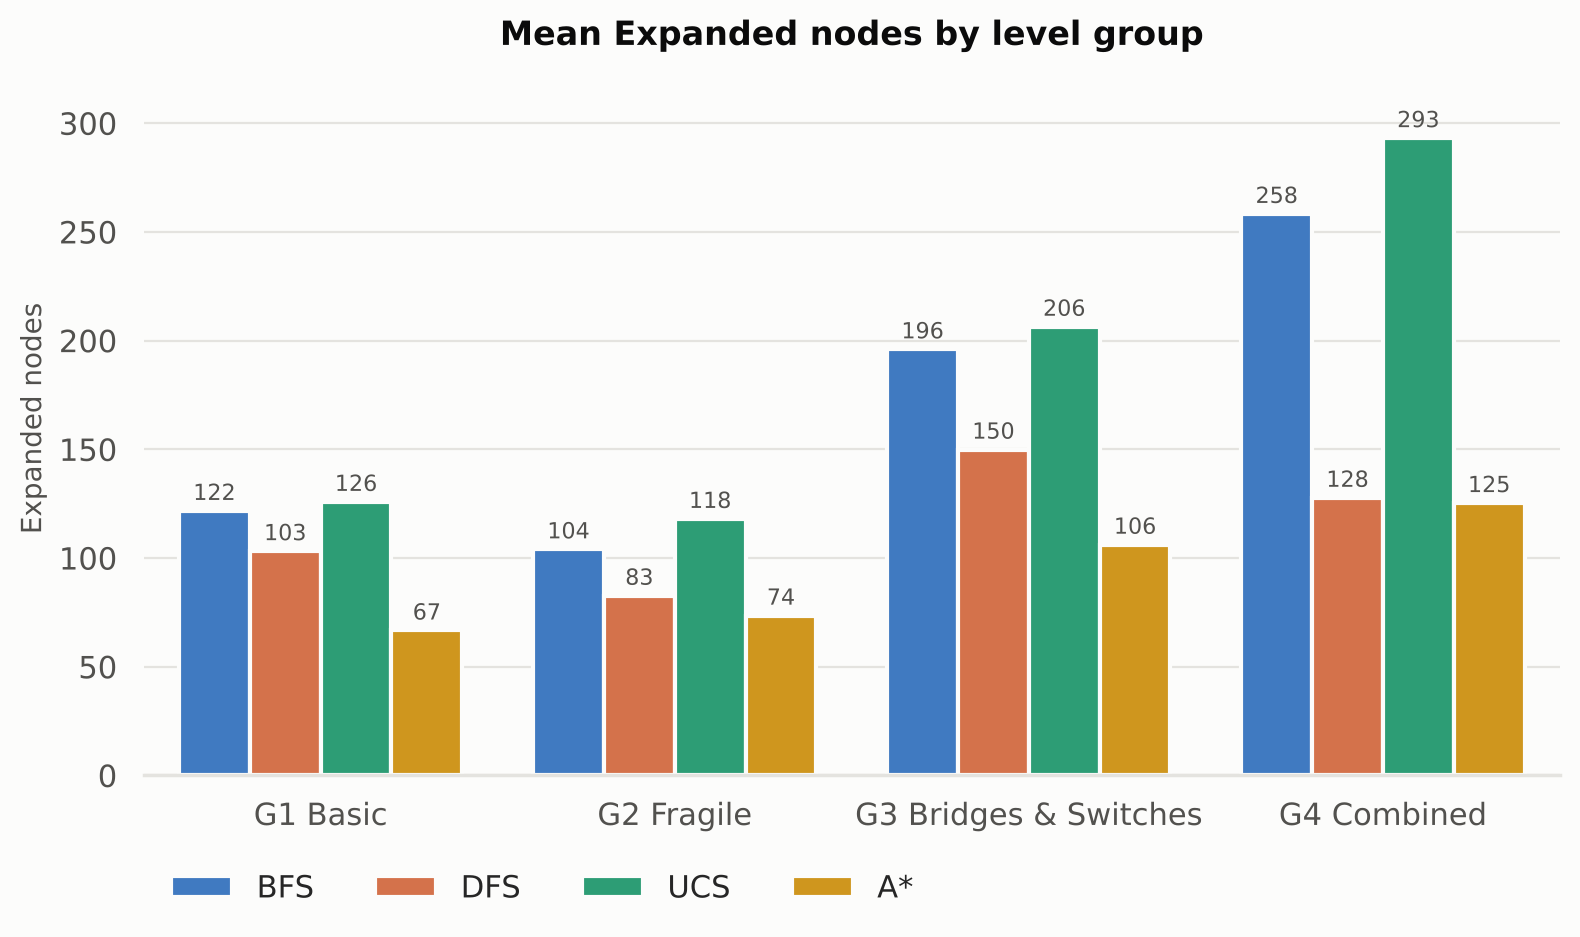
\includegraphics[width=\linewidth]{fig1c_expanded_by_group.png}
  \caption{Expanded nodes}
\end{subfigure}
\hfill
\begin{subfigure}{0.49\linewidth}
  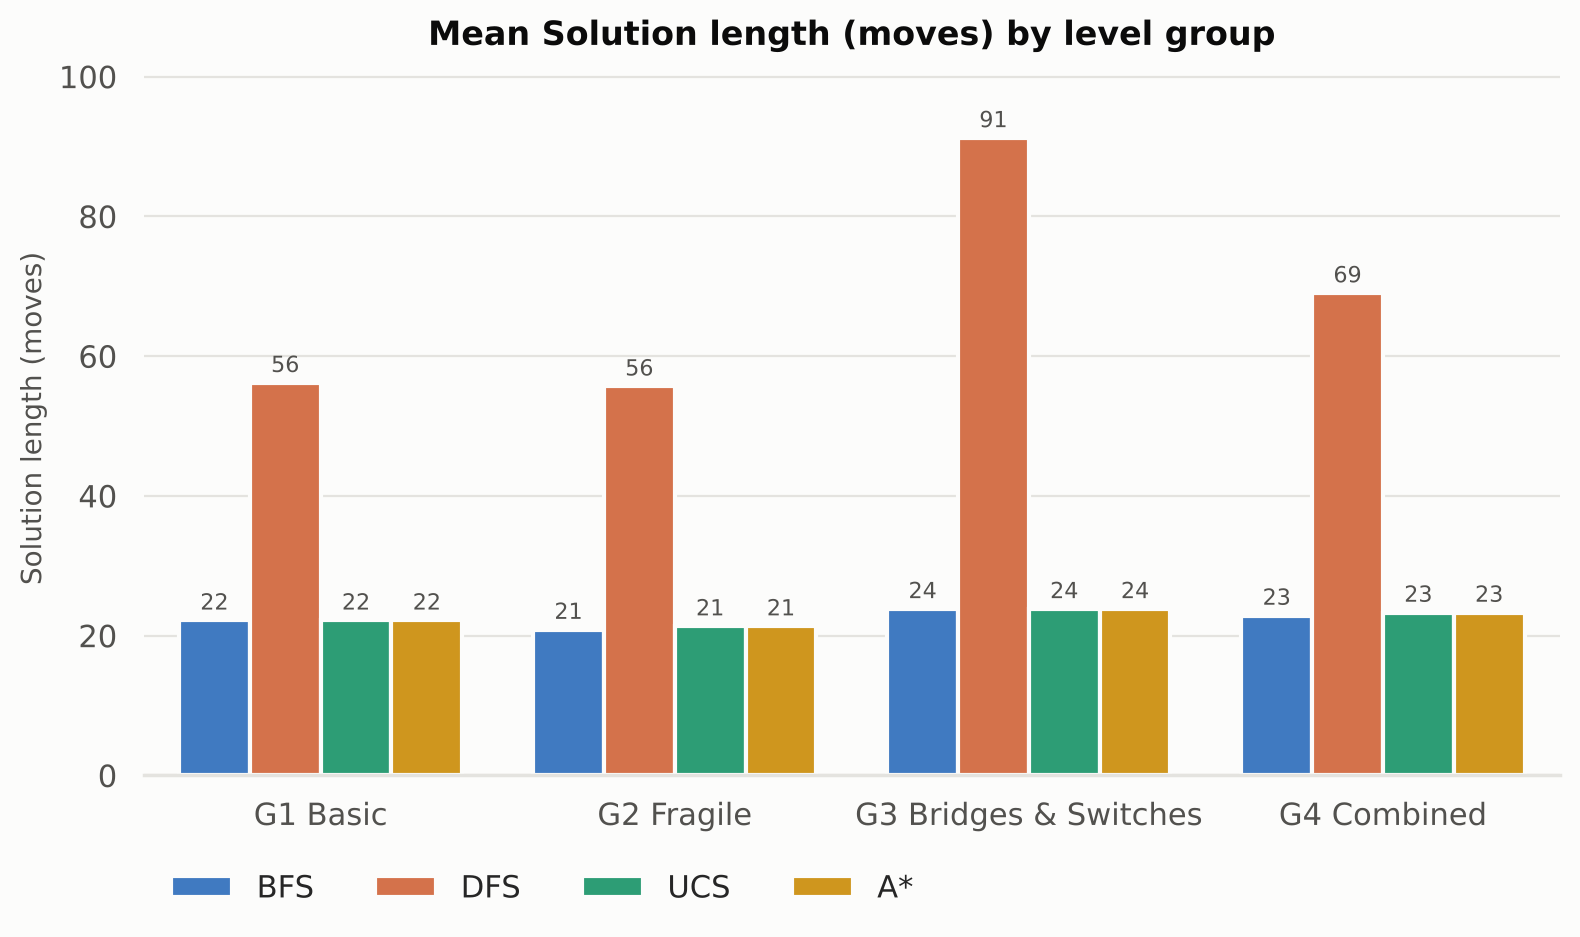
\includegraphics[width=\linewidth]{fig1d_moves_by_group.png}
  \caption{Solution length}
\end{subfigure}
\caption{Mean of the four metrics per test group}
\label{fig:groups}
\end{figure}

Figure~\ref{fig:groups}: from G1 to G4, the time, memory and expanded nodes of BFS and UCS roughly
double, because bridges multiply the state space by $2^B$. A* is lowest in time and expanded nodes
in every group. BFS, UCS and A* return solutions of almost the same length; DFS solutions are 2.5
to 4 times longer.

\begin{figure}[H]
\centering
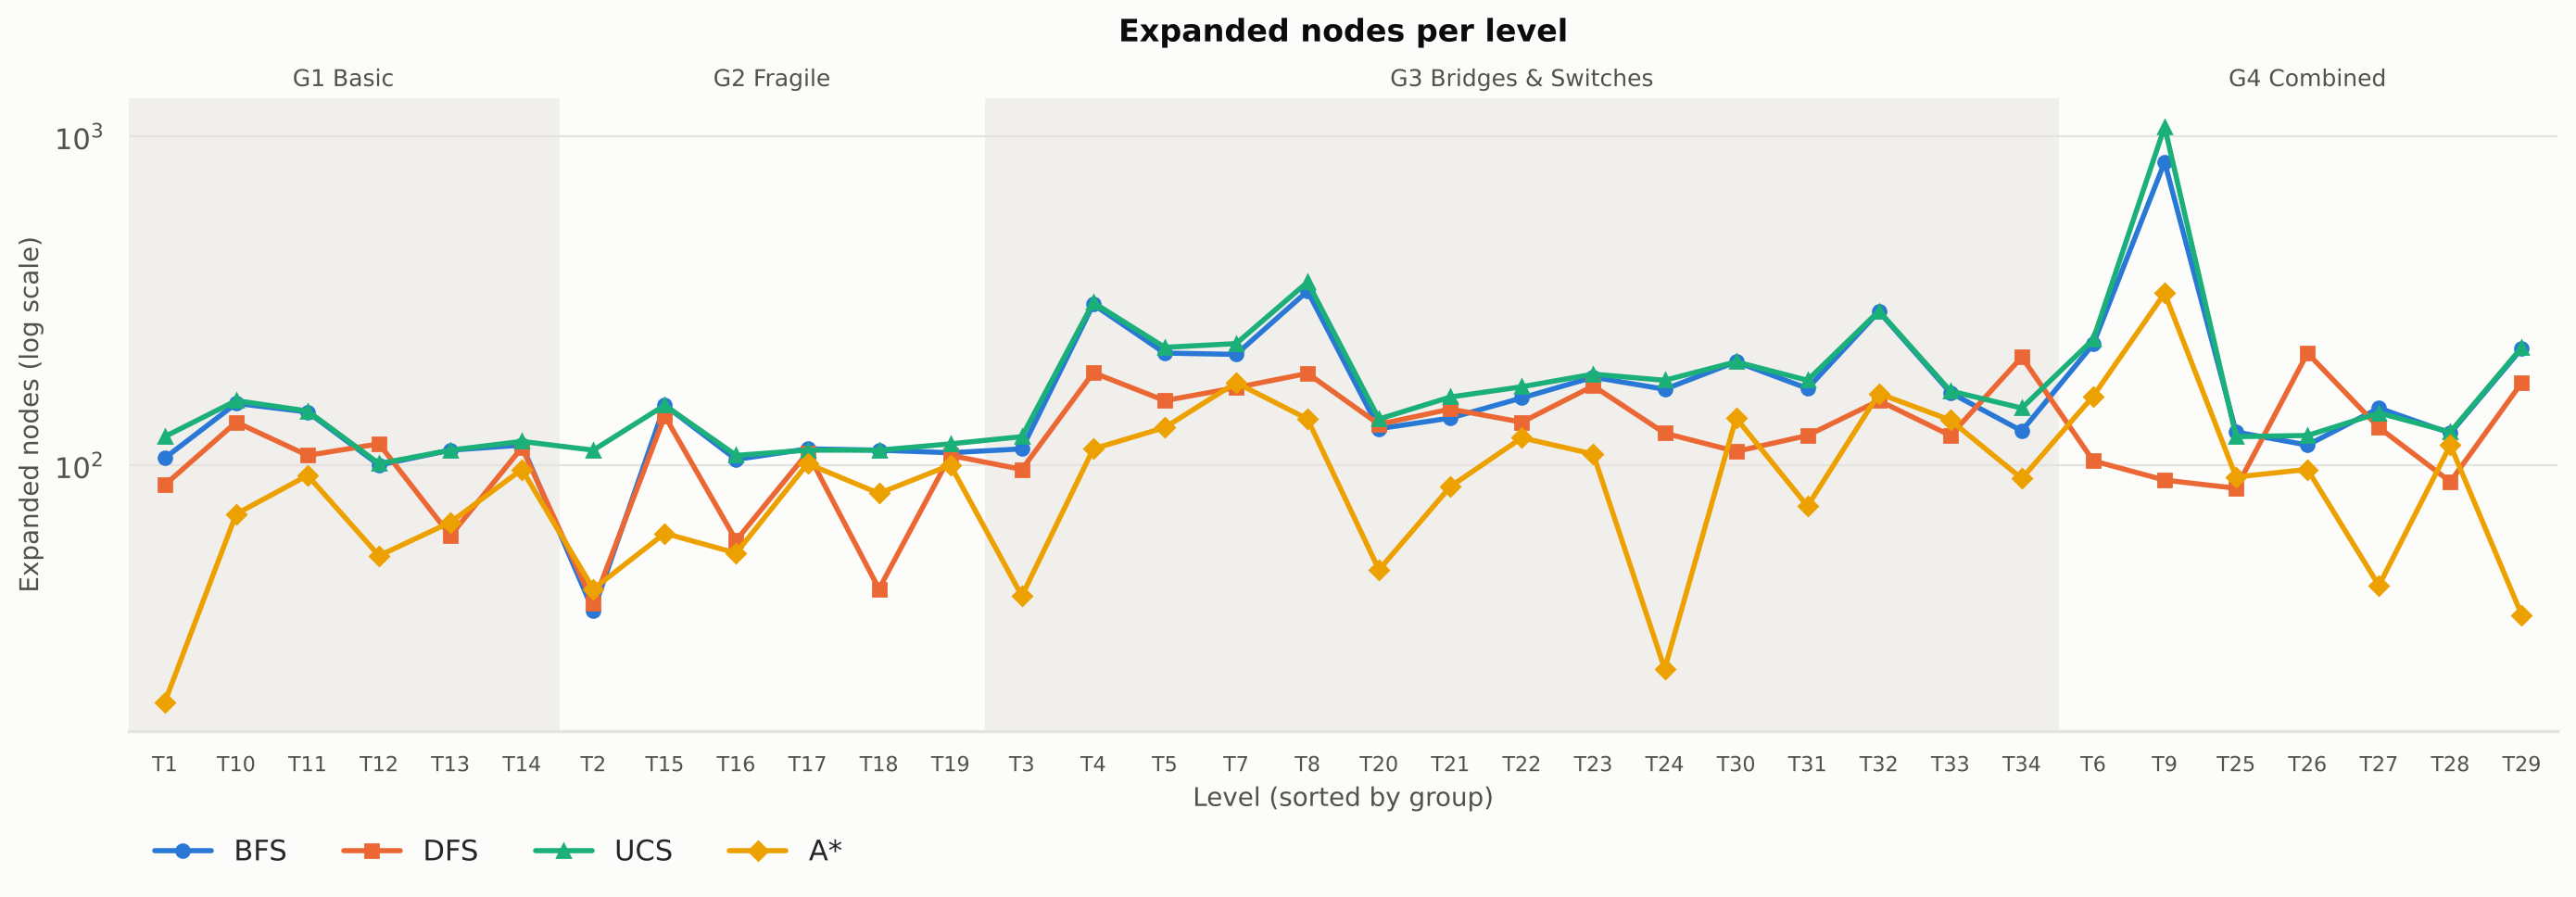
\includegraphics[width=\linewidth]{fig2_expanded_per_level.png}
\caption{Expanded nodes per stage (log scale), stages sorted by group}
\label{fig:perlevel}
\end{figure}

Figure~\ref{fig:perlevel}: the A* line lies below UCS on all 34 stages. BFS and UCS almost
coincide except on stages with fragile tiles. The largest peak is Test 9 (split switch), where BFS
and UCS expand 834 and 1068 states.

\begin{figure}[H]
\centering
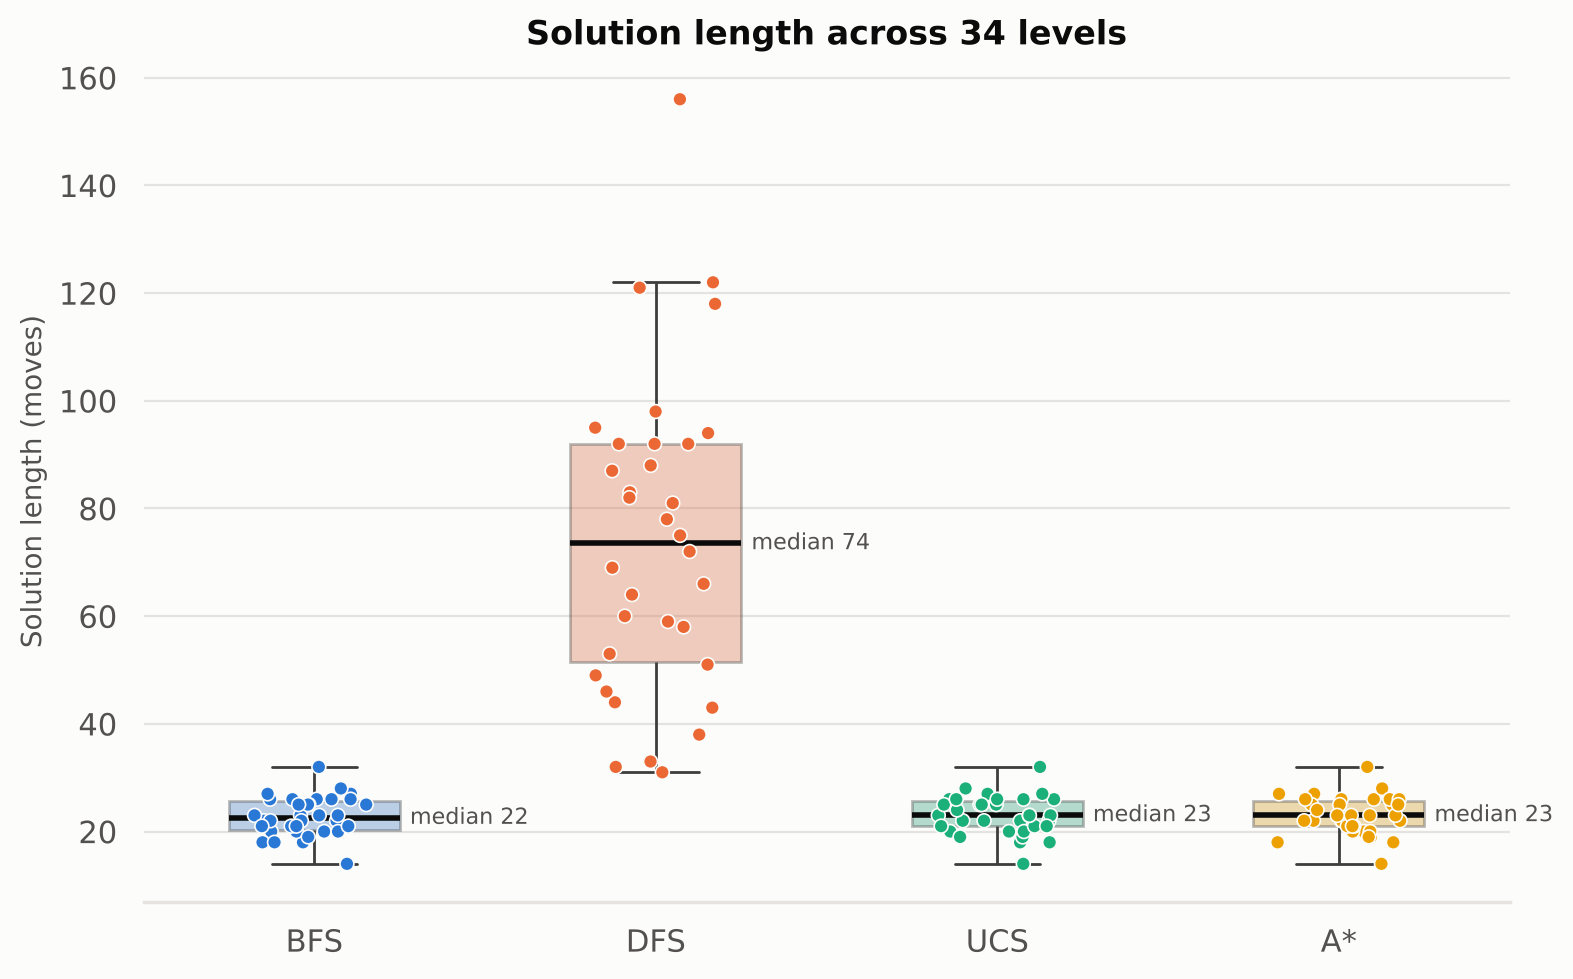
\includegraphics[width=0.75\linewidth]{fig3_moves_distribution.png}
\caption{Distribution of solution lengths over the 34 stages}
\label{fig:moves}
\end{figure}

Figure~\ref{fig:moves}: BFS, UCS and A* cluster around 22--23 moves, while DFS ranges from 31 to
156 moves (Test 4), with a median of 74.

\begin{figure}[H]
\centering
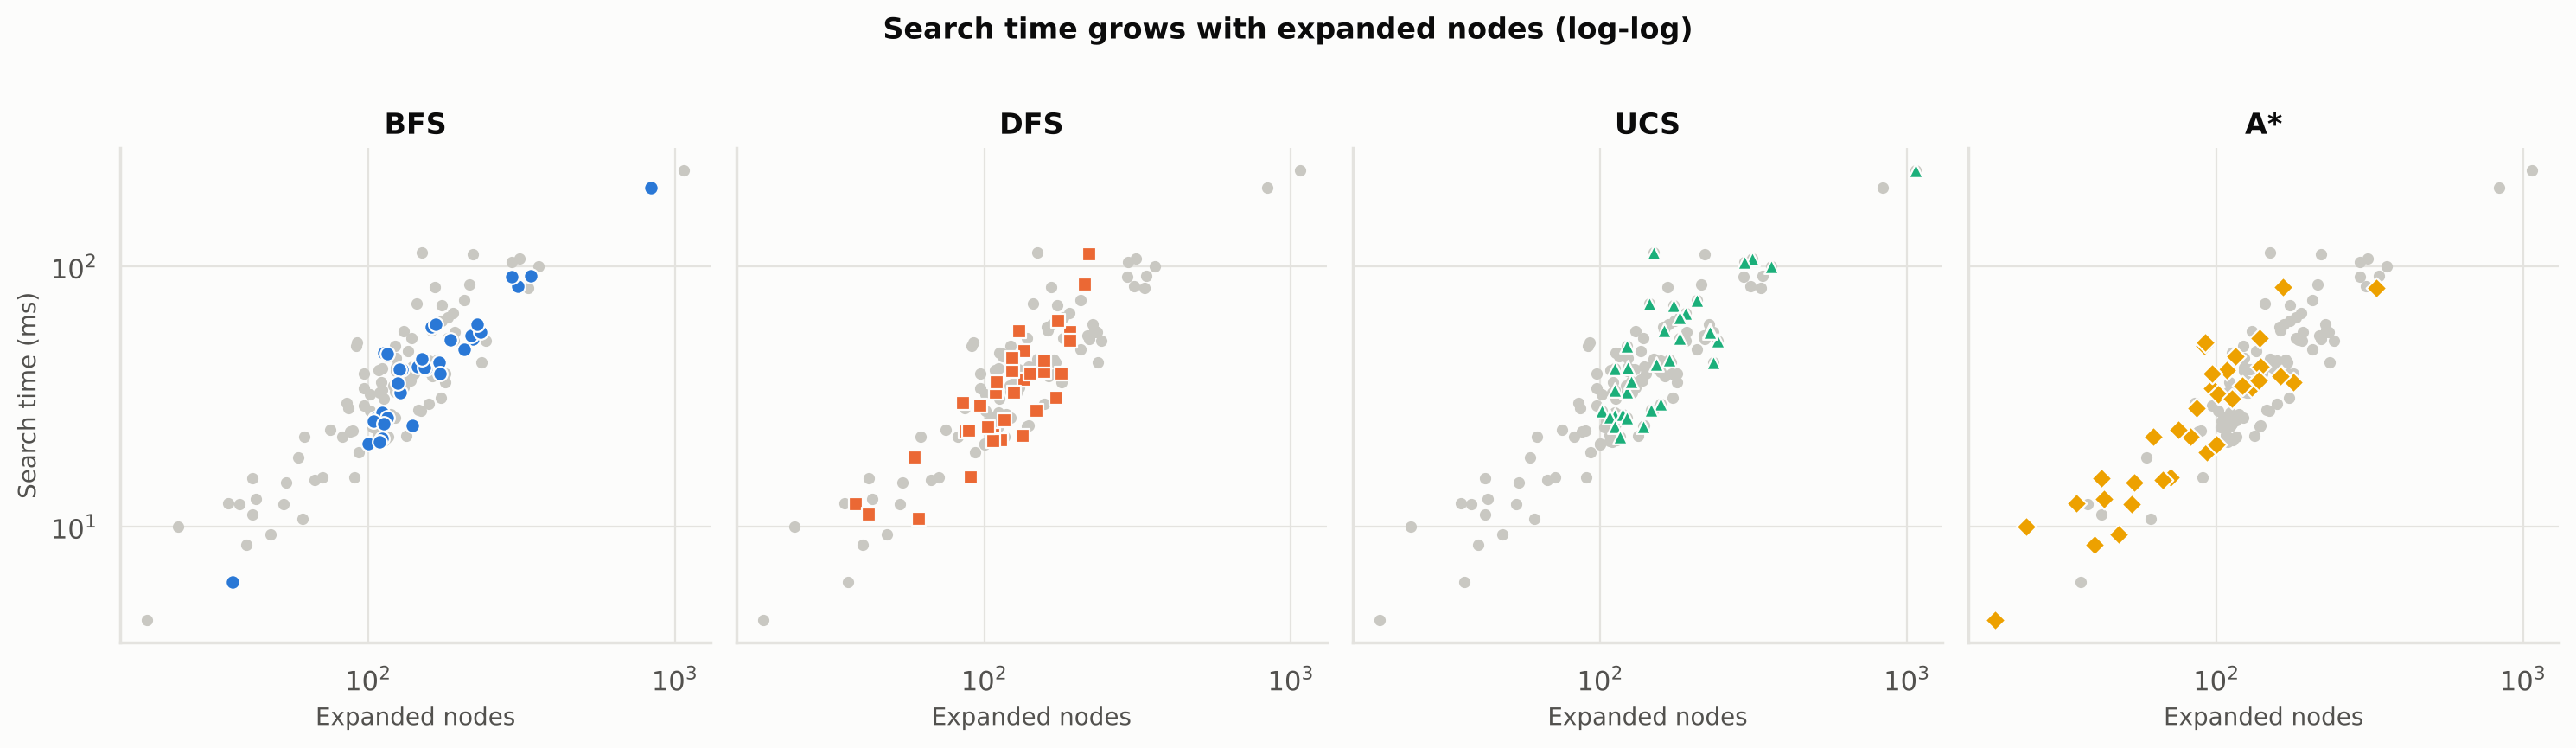
\includegraphics[width=\linewidth]{fig4_time_vs_expanded.png}
\caption{Search time against expanded nodes (log--log), one panel per algorithm}
\label{fig:timeexp}
\end{figure}

Figure~\ref{fig:timeexp}: the points lie close to a straight line (correlation 0.90 between log
time and log expanded nodes), so search time is driven mainly by the number of expansions. For the
same number of expansions, UCS and A* are slightly slower than BFS and DFS because each heap
operation costs $O(\log n)$ and A* also evaluates the heuristic.

\begin{figure}[H]
\centering
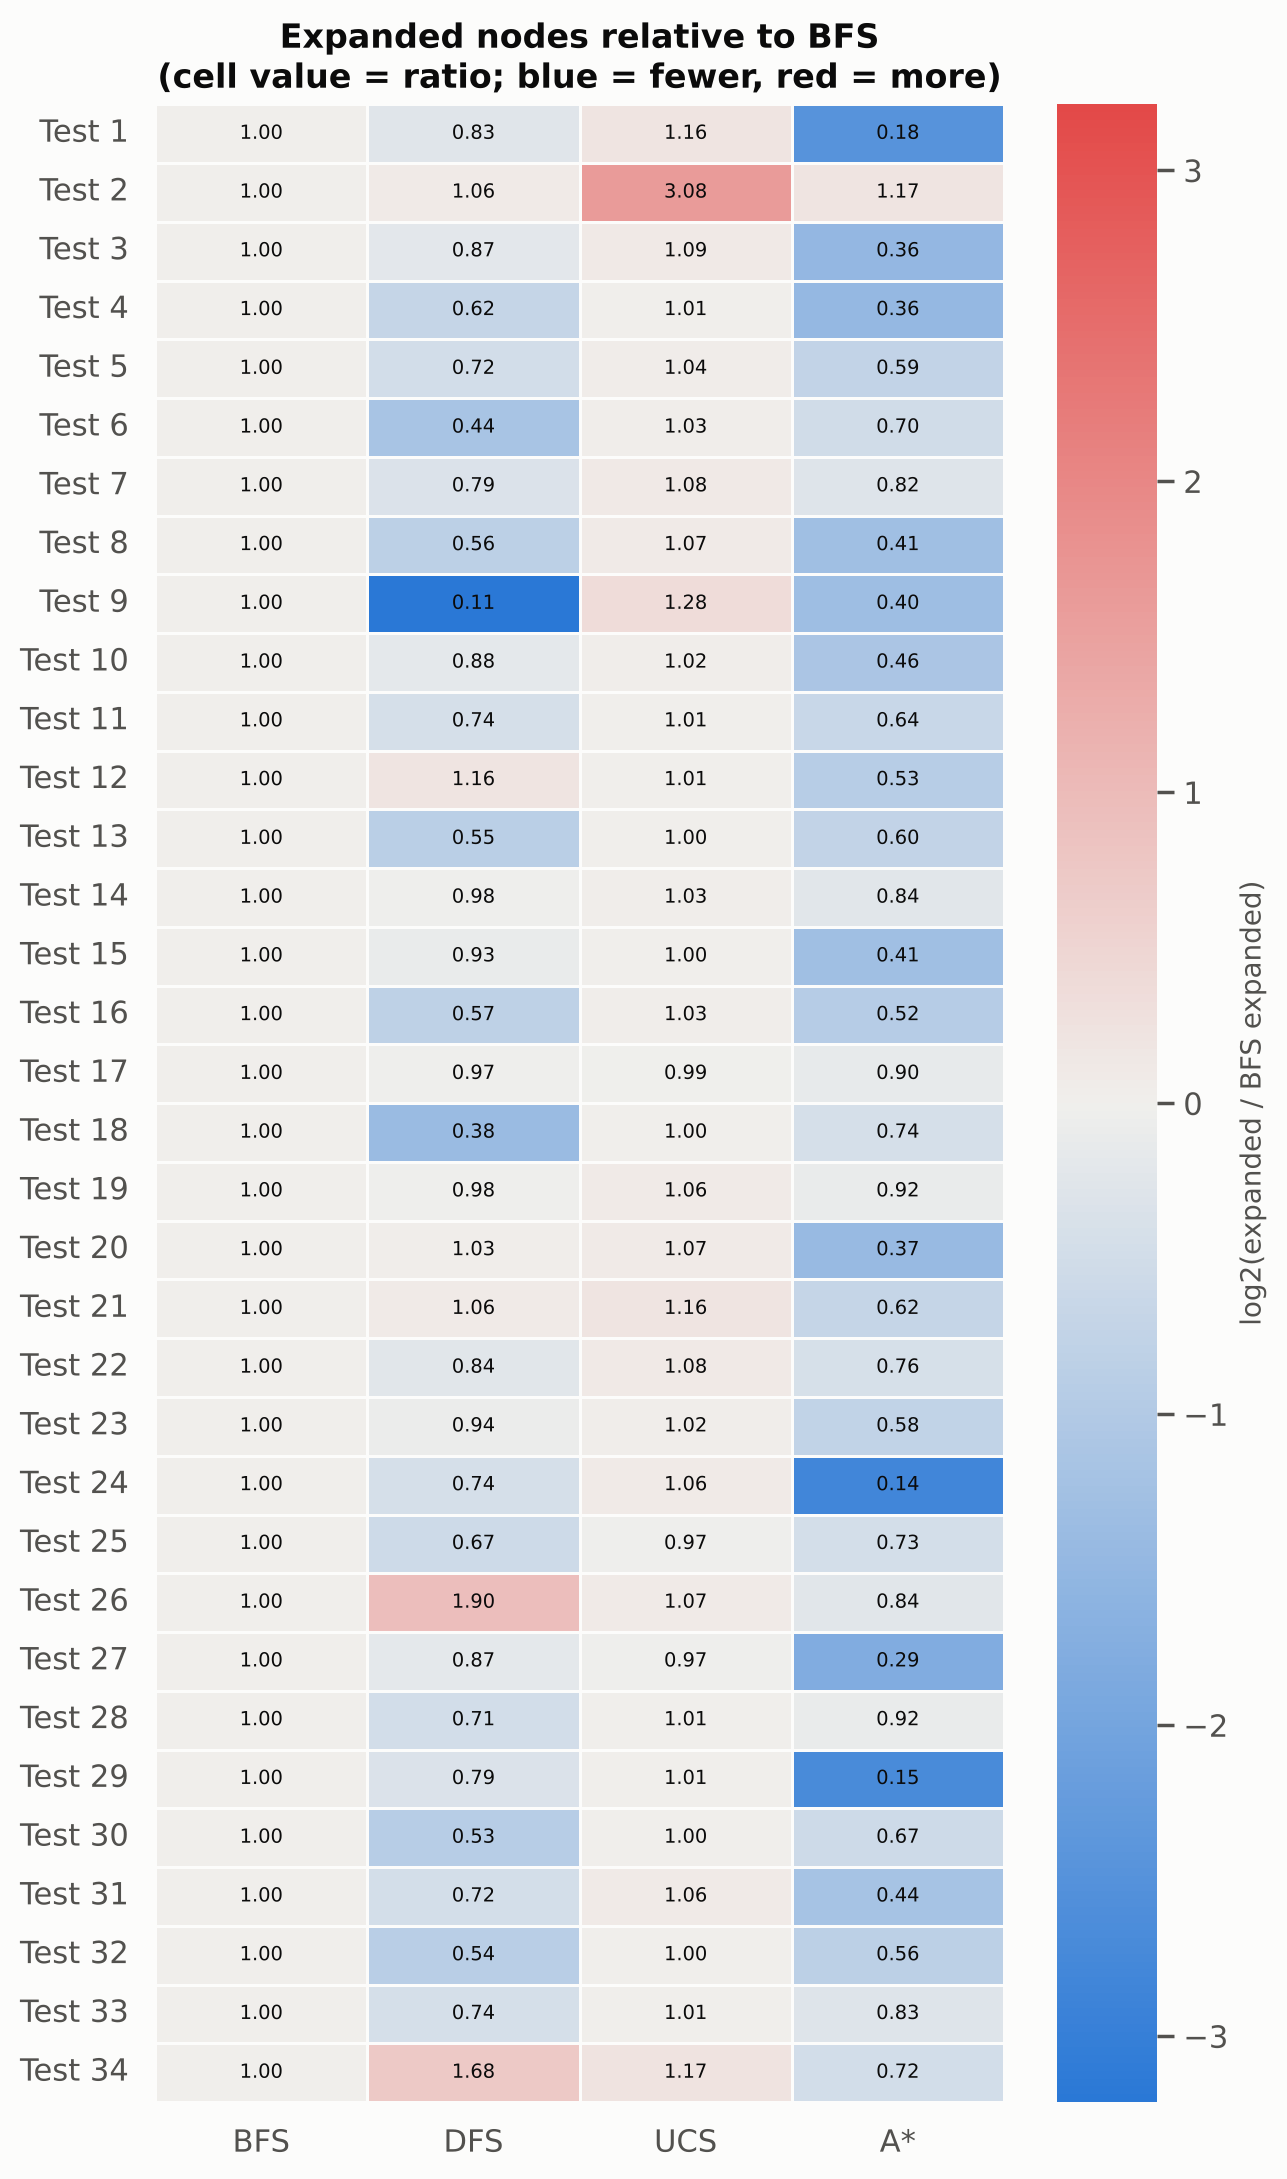
\includegraphics[width=0.62\linewidth]{fig5_expanded_ratio_heatmap.png}
\caption{Expanded nodes relative to BFS on the same stage (blue: fewer, red: more)}
\label{fig:heatmap}
\end{figure}

Figure~\ref{fig:heatmap}: A* expands fewer states than BFS on 33 of 34 stages (best: 0.14 on Test 24
and 0.18 on Test 1). UCS expands slightly more than BFS on 27 of 34 stages; Test 2 stands out with a
ratio of 3.08, explained in Section~\ref{sec:discussion}.

\begin{figure}[H]
\centering
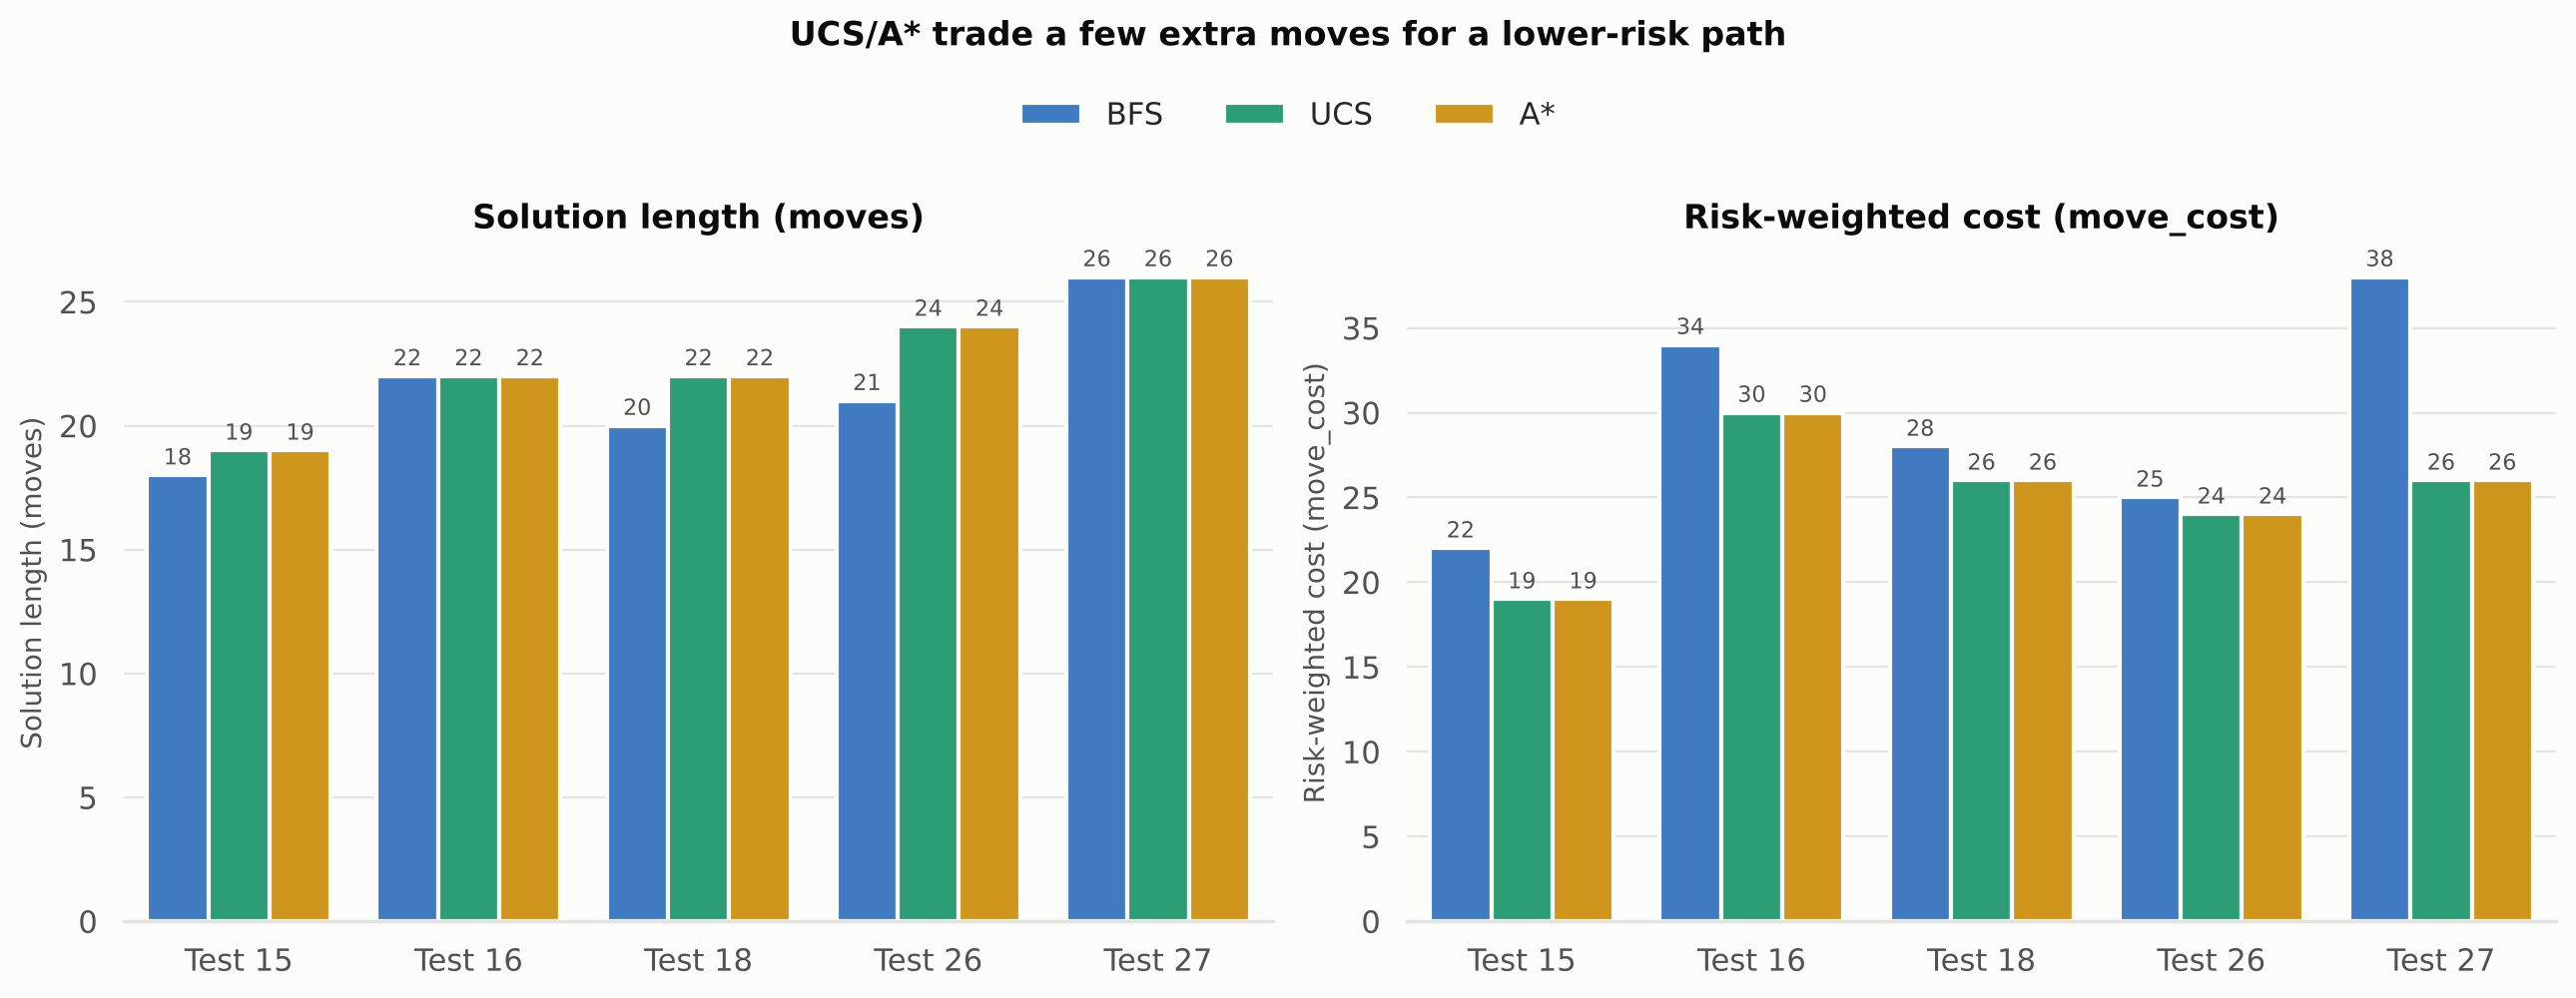
\includegraphics[width=\linewidth]{fig6_risk_tradeoff.png}
\caption{Stages where UCS/A* choose a different path from BFS: moves and risk cost}
\label{fig:risk}
\end{figure}

Figure~\ref{fig:risk}: on five stages UCS and A* pick a safer path than BFS. On Tests 15, 18 and 26
they take 1 to 3 extra moves to lower the risk cost; on Test 27 the path has the same 26 moves but
its cost drops from 38 to 26, avoiding all three fragile landings of the BFS path.

\subsection{Discussion}
\label{sec:discussion}

\textbf{Solution quality.} BFS, UCS and A* all return short solutions (22.8 to 23.0 moves on
average). UCS and A* return the same cost on all 34 stages, as theory predicts: both are optimal for
\texttt{move\_cost} and the heuristic is consistent. Compared with BFS they take only 0.18 extra
moves on average, but their risk cost is strictly lower on five stages (Tests 15, 16, 18, 26, 27).
On the other 29 stages the shortest path crosses no fragile tile, so any risk-based cost agrees
with BFS. DFS paths are on average 3.34 times longer than BFS paths (up to 7.1 times on a single
stage, and 1363 against 84 moves on Test All).

\textbf{Expanded nodes.} A* expands fewer states than UCS on every stage, 45\% fewer on average
(from 8.7\% on Test 28 to 86.7\% on Test 24). The heuristic helps most when the real path is close
to the straight line to the goal (Tests 1, 24, 29) and least on winding maps or around fragile tiles
(Tests 28, 17 and 19, only 9--14\% fewer). Over all four algorithms, A* expands the fewest states on 23 of
34 stages. UCS expands more than BFS on 27 stages for two reasons: BFS stops when the goal is
\emph{generated} while UCS waits until it is \emph{popped}, and the fragile penalty widens UCS's cost
contours. Test 2 is the extreme case: its solution must cross a fragile tile (cost 22 for 18 moves),
so UCS has to expand every state cheaper than 22, including states 19 to 21 moves deep that BFS never
reaches (111 against 36 expansions). DFS expands fewer states than BFS on 28 stages because it dives
deep and meets the goal early, at the price of very long paths.

\textbf{Time.} Time follows expanded nodes (Figure~\ref{fig:timeexp}). On average A* is fastest
(30 ms, fastest on 20 of 34 stages), then DFS (36 ms), BFS (48 ms) and UCS (56 ms). On Test All, DFS
is fastest (138 ms) because it expands the fewest states, and A* is second (188 ms).

\textbf{Memory.} UCS uses the most memory (highest on 32 of 34 stages): besides \texttt{parents} it
keeps \texttt{best}, \texttt{closed} and a heap that also holds stale entries. A* keeps the same
structures but expands far fewer states, so its memory is close to BFS. DFS uses the least memory on
16 of 34 stages. On Test All: UCS 2.5 MB, BFS 1.4 MB, A* 0.9 MB, DFS 0.8 MB.

\textbf{Effect of difficulty.} Bridges and switches (G3, G4) increase the work more than fragile
tiles (G2): each bridge group doubles the number of possible configurations, whereas fragile tiles
only forbid some standing placements. Split switches (Test 9, Test All) create the largest state
spaces because the two cubes move independently.

\begin{table}[H]
\centering
\caption{Strengths and weaknesses}
\label{tab:proscons}
\begin{tabularx}{\linewidth}{lXX}
\toprule
\textbf{Algorithm} & \textbf{Strengths} & \textbf{Weaknesses} \\
\midrule
BFS & Simple; optimal in the number of actions; stops as soon as the goal is generated & Ignores risk; expands and stores many states; not move-optimal when \texttt{SWAP} is used \\
DFS & Fewer expansions than BFS on 28/34 stages; least memory on 16/34; fastest on Test All & Solutions 3.3 times longer on average (16 times on Test All); result depends on the order in which actions are tried \\
UCS & Optimal for any non-negative cost; needs no heuristic; avoids fragile tiles & Slowest and most memory-hungry; extra expansions when the solution is expensive \\
A* & Same optimal cost as UCS with about 45\% fewer expansions; fastest on average & Needs a carefully designed and proven heuristic; weak on winding maps \\
\bottomrule
\end{tabularx}
\end{table}

\subsection{Limitations}

\begin{itemize}[leftmargin=*]
\item Each configuration was run once; averaging several runs would reduce timing noise.
\item \texttt{tracemalloc} slows Python down, so absolute times are higher than in the GUI.
\item The generated stages have similar sizes ($12\times25$) and goals usually on the right; Test All
complements them with a much larger map.
\item All runs start from the stage's initial state, not from mid-level states.
\end{itemize}

\section{Demo Video}

Public YouTube link: \fillin{https://youtu.be/...}

The video (with \fillin{English / Vietnamese} \fillin{subtitles / narration}) shows:
\begin{enumerate}[leftmargin=*]
\item \textbf{Graphical interface:} the board with every tile type (floor, void, goal, fragile,
soft/heavy/split switches and bridges), the block standing, lying horizontally and lying
vertically, and the control buttons (New Game, Restart, BFS, DFS, UCS, A*).
\item \textbf{Manual play:} rolling the block, pressing a switch to open a bridge, splitting and
merging the block, losing by falling off the board, and winning a stage.
\item \textbf{Solvers:} choosing a stage, running BFS, DFS, UCS and A*, reading the results card
(search time, memory, expanded nodes, solution length) and replaying the solution.
\end{enumerate}


% References
\clearpage
\bibliographystyle{plain}
\bibliography{ref/ref}
\nocite{*}


% Appendix
\appendix
\section{Per-stage results}
\label{app:perlevel}

Results from \texttt{experiments/summary\_4\_metrics.csv}, one run per algorithm and stage.

\begingroup
\renewcommand{\baselinestretch}{1.0}\small
\begin{longtable}{llrrrrrrrr}
\caption{Expanded nodes and solution length (moves) per stage}\label{tab:perlevel-exp}\\
\toprule
 & & \multicolumn{4}{c}{\textbf{Expanded nodes}} & \multicolumn{4}{c}{\textbf{Moves}} \\
\cmidrule(lr){3-6}\cmidrule(lr){7-10}
\textbf{Stage} & \textbf{Group} & BFS & DFS & UCS & A* & BFS & DFS & UCS & A* \\
\midrule
\endfirsthead
\toprule
\textbf{Stage} & \textbf{Group} & BFS & DFS & UCS & A* & BFS & DFS & UCS & A* \\
\midrule
\endhead
\bottomrule
\endfoot
Test 1 & G1 & 105 & 87 & 122 & 19 & 14 & 78 & 14 & 14 \\
Test 2 & G2 & 36 & 38 & 111 & 42 & 18 & 33 & 18 & 18 \\
Test 3 & G3 & 112 & 97 & 122 & 40 & 23 & 72 & 23 & 23 \\
Test 4 & G3 & 308 & 191 & 312 & 112 & 22 & 156 & 22 & 22 \\
Test 5 & G3 & 219 & 157 & 228 & 130 & 22 & 94 & 22 & 22 \\
Test 6 & G4 & 233 & 103 & 241 & 162 & 25 & 82 & 25 & 25 \\
Test 7 & G3 & 217 & 172 & 234 & 178 & 27 & 121 & 27 & 27 \\
Test 8 & G3 & 338 & 190 & 360 & 138 & 25 & 95 & 25 & 25 \\
Test 9 & G4 & 834 & 90 & 1068 & 333 & 21 & 75 & 21 & 21 \\
Test 10 & G1 & 154 & 135 & 157 & 71 & 26 & 87 & 26 & 26 \\
Test 11 & G1 & 145 & 107 & 146 & 93 & 22 & 53 & 22 & 22 \\
Test 12 & G1 & 100 & 116 & 101 & 53 & 20 & 43 & 20 & 20 \\
Test 13 & G1 & 111 & 61 & 111 & 67 & 26 & 44 & 26 & 26 \\
Test 14 & G1 & 115 & 113 & 118 & 97 & 25 & 32 & 25 & 25 \\
Test 15 & G2 & 152 & 141 & 152 & 62 & 18 & 98 & 19 & 19 \\
Test 16 & G2 & 104 & 59 & 107 & 54 & 22 & 51 & 22 & 22 \\
Test 17 & G2 & 112 & 109 & 111 & 101 & 27 & 31 & 27 & 27 \\
Test 18 & G2 & 111 & 42 & 111 & 82 & 20 & 38 & 22 & 22 \\
Test 19 & G2 & 109 & 107 & 116 & 100 & 20 & 83 & 20 & 20 \\
Test 20 & G3 & 129 & 133 & 138 & 48 & 21 & 46 & 21 & 21 \\
Test 21 & G3 & 139 & 148 & 161 & 86 & 23 & 92 & 23 & 23 \\
Test 22 & G3 & 160 & 135 & 173 & 121 & 28 & 60 & 28 & 28 \\
Test 23 & G3 & 185 & 174 & 189 & 108 & 26 & 92 & 26 & 26 \\
Test 24 & G3 & 170 & 125 & 181 & 24 & 20 & 69 & 20 & 20 \\
Test 25 & G4 & 126 & 85 & 122 & 92 & 25 & 66 & 25 & 25 \\
Test 26 & G4 & 115 & 219 & 123 & 97 & 21 & 59 & 24 & 24 \\
Test 27 & G4 & 149 & 130 & 144 & 43 & 26 & 64 & 26 & 26 \\
Test 28 & G4 & 125 & 89 & 126 & 115 & 19 & 49 & 19 & 19 \\
Test 29 & G4 & 226 & 178 & 228 & 35 & 23 & 88 & 23 & 23 \\
Test 30 & G3 & 206 & 110 & 206 & 139 & 26 & 81 & 26 & 26 \\
Test 31 & G3 & 171 & 123 & 181 & 75 & 21 & 92 & 21 & 21 \\
Test 32 & G3 & 293 & 157 & 294 & 165 & 23 & 122 & 23 & 23 \\
Test 33 & G3 & 166 & 123 & 168 & 137 & 32 & 58 & 32 & 32 \\
Test 34 & G3 & 127 & 213 & 149 & 91 & 18 & 118 & 18 & 18 \\
\end{longtable}

\begin{longtable}{lrrrrrrrr}
\caption{Search time (ms) and peak memory (KB) per stage}\label{tab:perlevel-time}\\
\toprule
 & \multicolumn{4}{c}{\textbf{Search time (ms)}} & \multicolumn{4}{c}{\textbf{Peak memory (KB)}} \\
\cmidrule(lr){2-5}\cmidrule(lr){6-9}
\textbf{Stage} & BFS & DFS & UCS & A* & BFS & DFS & UCS & A* \\
\midrule
\endfirsthead
\toprule
\textbf{Stage} & BFS & DFS & UCS & A* & BFS & DFS & UCS & A* \\
\midrule
\endhead
\bottomrule
\endfoot
Test 1 & 26.1 & 23.3 & 33.0 & 4.4 & 25.4 & 27.7 & 36.1 & 9.6 \\
Test 2 & 6.1 & 12.2 & 40.6 & 15.4 & 9.2 & 8.9 & 32.5 & 14.6 \\
Test 3 & 24.9 & 29.2 & 26.2 & 8.5 & 20.9 & 20.2 & 34.2 & 14.0 \\
Test 4 & 84.0 & 55.9 & 107.3 & 31.1 & 53.9 & 45.5 & 95.5 & 38.8 \\
Test 5 & 52.6 & 39.4 & 56.8 & 34.3 & 38.1 & 29.7 & 54.8 & 38.6 \\
Test 6 & 55.9 & 24.0 & 51.9 & 37.8 & 39.5 & 23.5 & 56.3 & 53.4 \\
Test 7 & 54.0 & 31.2 & 42.7 & 35.7 & 38.8 & 41.2 & 56.6 & 53.0 \\
Test 8 & 91.9 & 51.9 & 100.1 & 52.8 & 68.5 & 39.1 & 118.5 & 52.3 \\
Test 9 & 199.9 & 15.4 & 232.8 & 82.2 & 183.0 & 18.2 & 255.9 & 105.8 \\
Test 10 & 40.6 & 36.7 & 29.6 & 15.5 & 25.0 & 25.5 & 36.7 & 24.6 \\
Test 11 & 41.1 & 22.5 & 28.1 & 19.3 & 23.9 & 21.7 & 35.4 & 33.4 \\
Test 12 & 20.8 & 25.5 & 27.8 & 12.2 & 18.5 & 21.1 & 30.1 & 15.1 \\
Test 13 & 27.4 & 10.7 & 26.7 & 15.1 & 19.5 & 12.3 & 31.1 & 17.2 \\
Test 14 & 26.3 & 21.4 & 27.0 & 34.1 & 20.3 & 20.7 & 32.4 & 31.9 \\
Test 15 & 40.8 & 38.6 & 42.1 & 22.1 & 24.6 & 30.0 & 36.4 & 24.7 \\
Test 16 & 25.4 & 18.4 & 26.3 & 14.8 & 20.0 & 12.6 & 32.1 & 15.4 \\
Test 17 & 46.5 & 32.8 & 33.4 & 32.1 & 19.9 & 19.8 & 31.4 & 31.4 \\
Test 18 & 21.8 & 11.1 & 24.4 & 22.1 & 20.1 & 10.8 & 31.6 & 30.8 \\
Test 19 & 21.1 & 21.3 & 22.2 & 20.7 & 20.6 & 22.1 & 32.9 & 31.8 \\
Test 20 & 40.2 & 22.3 & 24.2 & 9.3 & 22.8 & 23.1 & 35.5 & 14.8 \\
Test 21 & 24.4 & 27.9 & 56.7 & 28.6 & 25.6 & 28.1 & 51.1 & 32.0 \\
Test 22 & 58.5 & 47.2 & 70.9 & 34.7 & 35.0 & 25.3 & 51.2 & 35.3 \\
Test 23 & 52.0 & 61.6 & 65.9 & 40.0 & 34.9 & 40.2 & 51.1 & 35.0 \\
Test 24 & 42.7 & 32.7 & 52.8 & 10.0 & 35.0 & 24.5 & 51.3 & 10.1 \\
Test 25 & 40.1 & 29.9 & 49.2 & 50.9 & 22.0 & 20.0 & 33.4 & 30.2 \\
Test 26 & 46.3 & 111.6 & 40.8 & 38.7 & 21.0 & 39.0 & 33.6 & 31.0 \\
Test 27 & 44.2 & 56.1 & 71.6 & 12.8 & 25.1 & 23.8 & 37.0 & 14.7 \\
Test 28 & 35.5 & 23.4 & 36.1 & 45.0 & 21.3 & 20.3 & 32.9 & 33.3 \\
Test 29 & 60.0 & 38.6 & 56.0 & 12.3 & 38.7 & 39.0 & 55.3 & 13.4 \\
Test 30 & 47.8 & 35.8 & 74.0 & 41.0 & 35.2 & 21.7 & 51.2 & 38.4 \\
Test 31 & 38.6 & 39.7 & 63.7 & 23.5 & 35.0 & 25.0 & 51.2 & 24.5 \\
Test 32 & 91.2 & 43.4 & 104.0 & 83.0 & 45.7 & 32.3 & 62.1 & 53.2 \\
Test 33 & 59.7 & 44.5 & 43.8 & 36.3 & 26.3 & 22.7 & 51.1 & 36.1 \\
Test 34 & 32.7 & 85.1 & 112.6 & 49.3 & 24.1 & 45.0 & 51.2 & 34.0 \\
\end{longtable}
\endgroup

\section{Running the source code and the experiments}

\begin{lstlisting}[language=bash, numbers=none]
# Game (from the Source/ folder)
python -m pip install -r requirements.txt
python main.py

# Experiments and charts (from the repository root)
python -m pip install pandas matplotlib seaborn
python experiments/run_experiments.py   # results CSV
python experiments/plot_results.py      # charts
\end{lstlisting}

\section{Use of Generative AI}

% TODO: describe honestly how your team used AI tools. Keep or delete the rows that apply.
\begin{table}[H]
\centering
\caption{Generative AI usage}
\label{tab:ai}
\begin{tabularx}{\linewidth}{lXX}
\toprule
\textbf{Tool} & \textbf{What it was used for} & \textbf{Example prompts} \\
\midrule
\fillin{Tool name} & \fillin{Task, e.g. debugging, explaining concepts, plotting code, report wording} & \fillin{Prompt} \\
\fillin{Tool name} & \fillin{Task} & \fillin{Prompt} \\
\bottomrule
\end{tabularx}
\end{table}

\fillin{Explain how the team checked and understood the AI-generated output before using it.}

\end{document}
